\documentclass[a4paper, 11pt, normalem]{report}

\usepackage{../../../LaTeX-Templates/Notes}
\usepackage{subfiles}

\title{Condensed Matter Physics \vspace{-20pt}}
\author{Prof Hatton and Dr Mendis}
\date{\vspace{-15pt}Epiphany Term 2019}
\rhead{\hyperlink{page.1}{Contents}}

\begin{document}

\maketitle
\tableofcontents

\part{}
%Hatton
\chapter{Free and Nearly Free Electrons}
\begin{wrapfigure}{r}{0.4\textwidth}
    \centering
    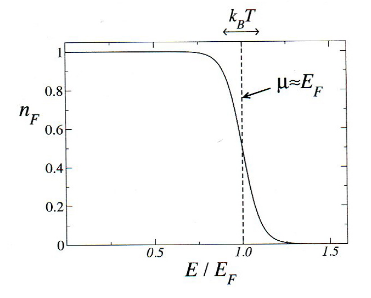
\includegraphics[width=0.4\textwidth]{fd.png}
\end{wrapfigure}
Given that electrons are fermions, we will use the Fermi-Dirac distribution. 
\begin{equation}
    n_F = \frac{1}{(e^{E-\mu/k_BT)}+1}
\end{equation}
We will consider electron waves in a box $V=L^3$ with periodic boundary conditions. 
The plane wavefunctions of the electron waves are of the form $e^{ik\cdot r}$ with wavevectors $(\frac{2\pi}{L})(n_1,n_2,n_3)$.
The plane waves have energies,
\begin{equation}
    E(k) = \frac{\hbar^2|k|^2}{2m}
\end{equation}
where $m$ is the electron mass. 

\begin{wrapfigure}{r}{0.4\textwidth}
    \centering
    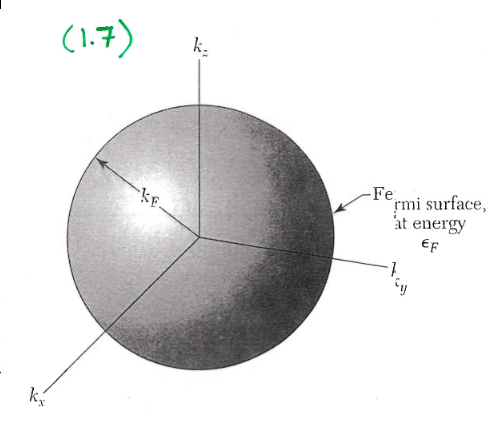
\includegraphics[width=0.4\textwidth]{fermisph.png}
\end{wrapfigure}
Thus the total number of electrons in the system is 
\begin{equation}
    N = 2\sum_k n_f\left(\frac{\e(k) - \mu}{k_BT}\right) = 2\frac{V}{(2\pi)^3}\int dk n_F\left(\frac{\e(k) - \mu}{k_BT}\right)
\end{equation}
where the prefactor of 2 accounts for the two possible spin states for each wavevector. 
We can define the Fermi energy as equal to $\mu$ at $T=0$.
\begin{equation}
    E_F = \frac{\hbar^2k_F^2}{2m}
\end{equation}
\begin{itemize}
    \item Fermi temperature, $T_F = \frac{E_F}{k_B}$
    \item Fermi momentum, $p_F = \hbar k_F$
    \item Fermi velocity, $v_F = \hbar k_F/m$
\end{itemize}
\begin{equation}
    N = 2\frac{V}{(2\pi)^3}\left(\frac{4}{3}\pi k_F^3\right)
\end{equation}
This plots a Fermi sphere.

At $T=0$, the electrons fill a sphere (the Fermi sphere) of radius $k_F$.
The surface of the sphere is known as the Fermi surface and delineates filled states from unfilled states. 
The density of free electrons,
\begin{align}
    n &= \frac{N}{V} \\
    \implies k_F &= (3\pi^2n)^{1/3} \\
    \implies E_F &= \frac{\hbar^2(3\pi^2n)^{2/3}}{2m}
\end{align}

Many problems with the Sommerfeld free electron theory, e.g. The Hall Effect
\begin{equation} 
    R_H = \frac{-1}{n_e}
\end{equation}
Sometimes too high (e.g. Bi), sometimes too low (e.g. Al).

The heat capacity of metals
\begin{equation}
    C = \gamma T + \alpha T^3
\end{equation}
does not have a zero intercept.
Values of $\gamma_{exp}$ vary from $0.2\gamma_{theory}$ to $50\gamma_{theory}$, suggesting that $m$, the electron mass, is a variable. 
\begin{figure}[H]
    \centering
    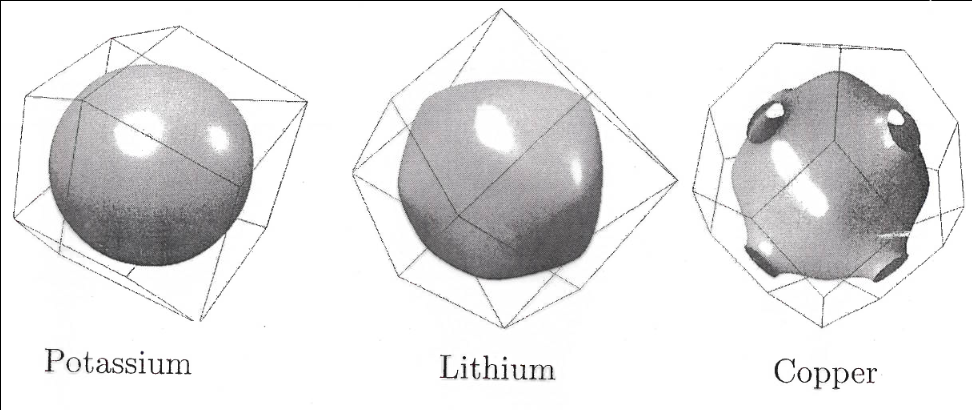
\includegraphics[scale=0.4]{spheres.png}
    \caption{Whilst some Fermi spheres are spherical (e.g. Potassium), others (e.g. Copper) are not}
\end{figure}

\chapter{}
Consider a one-dimensional chain of atoms with spacing $a$ between them. 
The figure below shows the low energy portion of the band structure for (a) free electrons, and (b) nearly-free electrons with an energy gap at $k = \pm \frac{\pi}{a}$.
\begin{figure}[H]
    \centering
    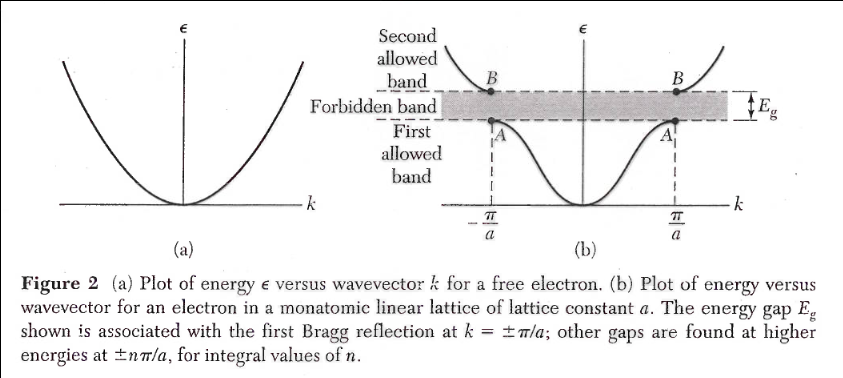
\includegraphics[scale=0.5]{brill.png}
\end{figure}
The Bragg condition $(k+G)^2 = k^2$ for diffraction of a wave of wavevector $k$ then becomes 
\begin{equation}
    l = \pm \frac{G}{2} = \pm \frac{n\pi}{a}
\end{equation}
where $G = \frac{2n\pi}{a}$ is a reciprocal lattice vector and $n$ is an integer.
The first reflections and the first energy gap occur at $k = \pm \frac{\pi}{a}$.
The region in k-space between $-\frac{\pi}{a}$ and $+\frac{\pi}{a}$ is the first Brillouin zone of the lattice.
Higher energy gaps occur for other values of $n$.

The wavefunctions at $\pm \frac{\pi}{a}$ of the form $\exp{(\pm i\pi x/a)}$ are not the plane travelling waves we might expect.
At these special values of $k$, the wavefunctions are made up of equal parts of waves traveling to the right, and waves traveling to the left. 
At the Brillouin zone boundaries, the wave is reflected back. 

The time-independent result is a standing wave.
We can form 2 different standing waves,
\begin{align}
    \Psi(+) &= \exp{\left(\frac{i\pi x}{a}\right)}  + \exp\left(\frac{-\pi x}{a}\right) = 2\cos\left(\frac{\pi x}{a}\right) \\
    \Psi(-) &= \exp\left(\frac{i\pi x}{a}\right) - \exp\left(\frac{-i\pi x}{a}\right) = 2i\sin\left(\frac{\pi x}{a}\right) 
\end{align}
The two standing waves $\Psi(+)$ and $\Psi(-)$ pile up electorn density in different regions, and have different energies. 
The probability density $P$ is $\Psi^*\Psi = |\Psi|^2$.
For a traveling plane wave, $P = \exp(-ikx)\exp(ikx) = 1$.
But $\Psi(+)$ has a density, 
\begin{equation}
    P(+) = |\Psi(x)|^2 \propto \cos^2\left(\frac{\pi x}{a}\right)
\end{equation}
This concentrates electron density at the postive ions. 
\begin{figure}[H]
    \centering
    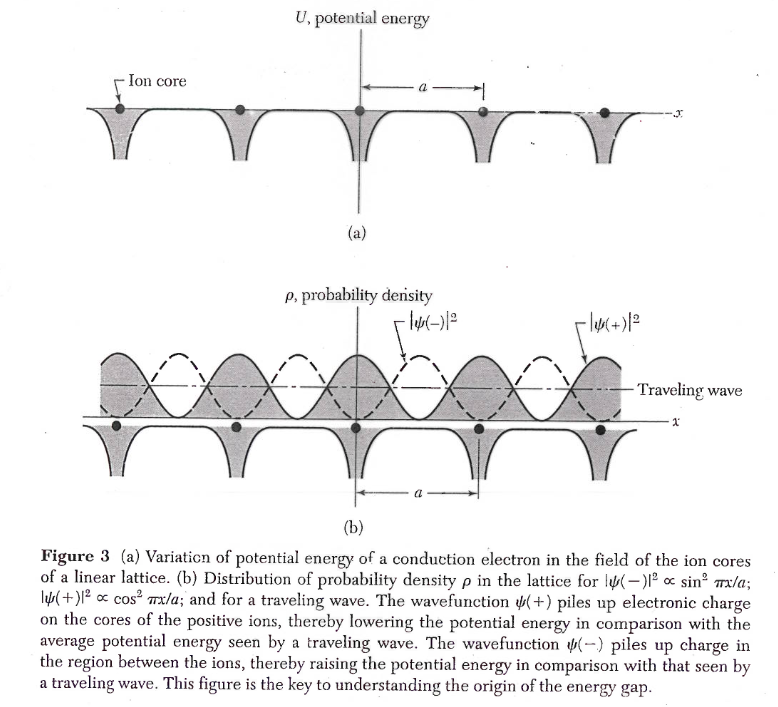
\includegraphics[scale=0.5]{l2f3.png}
\end{figure}
The standing wave $\Psi_+$ concentrates the electron density at the ion cores where the potential energy is at its lowest. 
This cause a lowering of the energy of $\Psi_+$.
For the other standing wave, $\Psi_-$, the probability density is
\begin{equation}
    P(-) = |\Psi|^2 \propto \sin^2\left(\frac{\pi x}{a}\right)
\end{equation}
which concentrate $e^-$ density between the positive ion cores - Bad News. 

Thus at the Brillouin zone boundary, 
\begin{equation}
    k = \big|\frac{\pi}{a}\big|
\end{equation}
The two standing waves exist with the same wavevector but different energies.

The wavefunctions at the Brillouin zone boundary $k=\frac{\pi}{a}$ are $\sqrt{2}\cos(\frac{\pi x}{a})$ and $\sqrt{2}\sin(\frac{\pi x}{a})$, normalised over unit length. 
If the PE of an electron in the one dimensional chain at point $x$ is
\begin{equation}
    U(x) = U\cos\left(\frac{2\pi x}{a}\right)
\end{equation}
Then the first-order energy different between the two standing waves is
\begin{align}
    E_g &= \int_0^1 dx ~ U(x) \left[|\Psi_+|^2 - |\Psi_-|^2\right] \\
        &= 2\int dx ~ U(x) \cos\left(\frac{2\pi x}{a}\right)\left(\cos^2\left(\frac{\pi x}{a}\right) - \sin^2\left(\frac{\pi x}{a}\right) \right) \\
        &= U
\end{align}
We see that the energy gap $E_g$ is equal to the Fourier component of the crystal potential.

\section{Model 2}
We will again start with plane electron waves perturbed by a periodic potential and use second-order perturbation theory from QM.

We start with completely free electrons whoes Hamiltonian is 
\begin{equation}
    \Ham_0 = \frac{p^2}{2m}
\end{equation}
The plane waves $|k\rangle$ have eigenenergies
\begin{equation}
    \e_0(k) = \frac{\hbar^2|k|^2}{2m}
\end{equation}
We consider a weak potential perturbation, 
\begin{equation}
    \Ham = \Ham_0 + V(r)
\end{equation}
with V periodic, $V(r) = V(r+R)$, where $R$ is any lattice vector.

The matrix elements of this potential are the Fourier components
\begin{equation}
    \langle k'|V|k\rangle = \frac{1}{L^3} \int dr~ e^{i(k-k')\cdot r} V(r) \equiv V_{k-k'}
\end{equation}
which is zero unless $k-k'$ is a reciprocal lattice vector. 

So any plane wave state $k$ can only scatter into another $k'$ if the two plane waves are separated by a reciprocal lattice vector.
Now, we apply the rules of perturbation theory. 
At first order, 
\begin{equation} 
    \e(k) = \e_0(k) + \langle k|V|k\rangle = \e_0(k) + V
\end{equation}
Just an energy shift. Assume $V_0 = 0$.

At second order, 
\begin{equation}
    \e(k) = \e_0(k) + \sum_{k'=k+G}' \frac{|\langle k'|V|k\rangle|^2}{\e_0(k) - \e_0(k')}
\end{equation}
where ' means the sum is restricted to have $G\neq 0$.
Be careful - for some $k'$ then $\e_0(k)$ may be very close to $\e_0(k')$. 
Then the sum will diverge. 
Therefore, we need degenerate perturbation theory. 
To see when this degenerate situation occurs, look for solutions of
\begin{align}
    \e_0(k) &= \e_0(k') \\
    k' = k+G
\end{align}
Let us return to our 1D case. 
Since $\e(k) \approx k^2$ then the only possible solution is 
\begin{equation}
    k' = -k
\end{equation}
This means the two equations are only satisfied for 
\begin{equation} 
    k' = -k = \frac{n\pi}{a} 
\end{equation}
Precisely on the Brillouin zone boundaries. 
This is generally true, in 1D, 2D, 3D, etc. 
So, when we are very near a zone boundary, our second order is divergent and we need degenerate perturbation theory. 
In this approach we diagonalise the Hamiltonian within the degenerate space first.

\section{Degenerate Perturbation Theory}
If our two plane wave states $|k\rangle$ and $|k'\rangle = |k+G\rangle$ are of approximate equal energy, then we diagonalise matrix elements first. 
We have
\begin{align}
    \langle k|H|k\rangle &= \e_0(k) \\
    \langle k'|H|k'\rangle &= \e_0(k') = \e_0(k+G) \\
    \langle k|H|k'\rangle &= V_{k-k'} = V^*_G \\
    \langle k'|H|k\rangle &= V_{k'-k} = V_G
\end{align}
Within this two-dimensional space, we can write any wavefunction as
\begin{equation}
    |\psi\rangle = \alpha|k\rangle + \beta|k'\rangle = \alpha|k\rangle + \beta|k+G\rangle
\end{equation}
Using the variational principle to minimise the energy is like solving the effective Schrodinger equation,
\begin{equation}
    \begin{pmatrix}
        \e_0(k) & V_G^* \\
        V_G & \e_0(k+G) 
    \end{pmatrix}
    \begin{pmatrix}
        \alpha \\
        \beta
    \end{pmatrix} = E
    \begin{pmatrix}
        \alpha \\
        \beta
    \end{pmatrix}.
\end{equation}
The characteristic equation determining $E$ is then
\begin{equation}
    [\e_0(k) - E][\e_0(k+G) - E] - |V_G|^2 = 0
\end{equation}

\section{Life at the Brillouin Zone Boundary}
\begin{wrapfigure}{r}{0.4\textwidth}
    \centering
    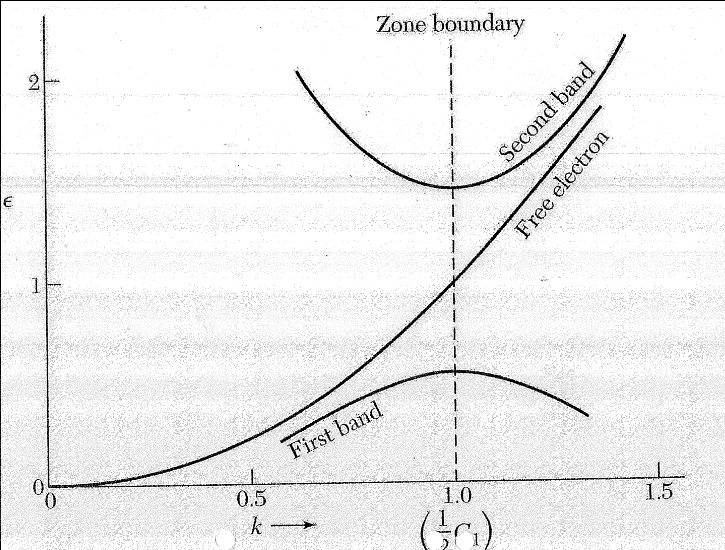
\includegraphics[width=0.4\textwidth]{boundary.png}
\end{wrapfigure}
At the Brillouin zone boundary, $k' = k+G$ and hence
\begin{equation}
    \e_0(k) = \e_0(k+G).
\end{equation}
Then the characteristic equation simplifies to
\begin{equation}
    [\e_0(k) - E]^2 = |V_G|^2
\end{equation}
or equivalently,
\begin{equation}
    E_{\pm} = \e_0(k) \pm |V_G|.
\end{equation}
Thus a gap opens up at the zone boundary. 
In the free electron theory, $k$ and $k'$ both had an energy, $\e_0(k)$. 

When we add a periodic potential, $V_G$, the two eigenstates form two linear combinations whose energies differ by $\pm |V_G|$.
Just like in Model 1.

\section{Nearly-free electron WFs in 1D}
To understand what the wavefunctions look like, let us retreat to our 1D chain of atoms. 
Let us assume we have a potential, 
\begin{equation}
    V(x) = \tilde{V}\cos\left(\frac{2\pi x}{a}\right),~ \tilde{V} > 0
\end{equation}
The Brillouin zone boundaries are at $k = \frac{\pi}{a}$ and $k' = -k = -\frac{\pi}{a}$ so that $k' -k = G = -\frac{2\pi}{a}$ and $\e_0(k) = \e_0(k')$.
Examining the effective Schrodinger equation, we discover that the solutions (when $\e_0(k) = \e_0(k')$) are given by $\alpha = \pm \beta$, which gives eigenstates, 
\begin{equation}
    |\psi_{\pm}| = \frac{1}{\sqrt{2}}(|k\rangle \pm |k'\rangle),
\end{equation}
corresponding to the eigenenergies, $E_\pm$.
We can write the real (direct) space version of these $|k\rangle$ wavefunctions as 
\begin{align}
    |k\rangle &\to e^{ikx} = e^{ik\pi/a} \\
    |k\rangle &\to e^{-ik'x} = e^{-ik'\pi/a}
\end{align}
Thus, the two eigenstates are given by
\begin{align}
    \psi_+ &\approx e^{ix\pi/a} + e^{-ix\pi/a} \\
           &\propto \cos\left(\frac{x\pi}{a}\right) \\
    \psi_- &\approx e^{ix\pi/a} - e^{-ix\pi/a} \\
           &\propto sin\left(\frac{x\pi}{a}\right)
\end{align}
And the densities $|\psi_\pm|^2$ associated with these two wavefunctions are shown - just like in Model 1.
\begin{figure}[H]
    \centering
    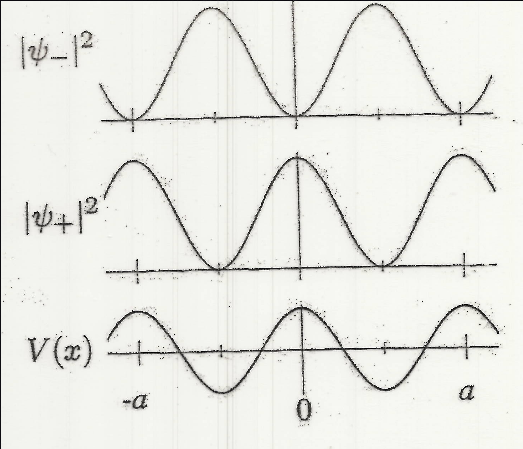
\includegraphics[scale=0.7]{fform.png}
\end{figure}
$\psi_+$ fits with the potential, slotting into the minima; $\psi_-$ goes against the potential, slotting into the maxima.

\chapter{}
\section{Life close to the Brillouin Zone Boundary}
Staying in one-dimension, we need only solve
\begin{equation}
    (\e_0(k) - E)(\e_0(k+G) - E) - |V_G|^2 = 0 
\end{equation}
in generality.
At $k = \pm\frac{n\pi}{a}$ separated by $G= \pm \frac{2n\pi}{a}$, this opened up gas $\pm|V_G|$ at the zone boundaries.

Now let us consider a plane wave near the zone boundary, $k = \frac{n\pi}{a} + \delta$ with $\delta$ being small. 
This wavevector can scatter into $k' = -\frac{n\pi}{a} + \delta$ via the reciprocal lattice vector, $G$.
Then, 
\begin{align}
    \e_0\left(\frac{n\pi}{a}+\delta\right) &= \frac{\hbar^2}{2m}\left[\left(\frac{n\pi}{a}\right)^2 + \frac{2n\pi\delta}{a} + \delta^2\right] \\
    \e_0\left(-\frac{n\pi}{a}+\delta\right) &= \frac{\hbar^2}{2m}\left[\left(\frac{n\pi}{a}\right)^2 - \frac{2n\pi\delta}{a} + \delta^2\right]
\end{align}
which simplifies to 
\begin{equation}
    \left\{\frac{\hbar^2}{2m}\left[\left(\frac{n\pi}{a}\right)^2 + \delta^2\right] - E\right\}^2 = \left\{\frac{\hbar^2}{2m}\frac{2n\pi\delta}{a}\right\}^2 + |V_G|^2
\end{equation}
or 
\begin{equation}
    E_\pm = \frac{\hbar^2}{2m}\left[\left(\frac{n\pi}{a}\right)^2 + \delta^2\right] \pm \sqrt{\left(\frac{\hbar^2}{2m}\frac{2n\pi\delta}{a}\right)^2+|V_G|^2}
\end{equation}
Expanding for the square root for small $\delta$ gives
\begin{equation}
    E_\pm = \frac{\hbar^2\left(\frac{n\pi}{a}\right)^2}{2m} \pm |V_G| + \frac{\hbar^2\delta^2}{2m}\left[\frac{1+\hbar^2\left(\frac{n\pi}{a}\right)^2}{m}\frac{1}{|V_G|}\right]
\end{equation}
For small perturbations, the second term in square brackets is greater than 1, so for one of the two solutions, the square bracket is negative.
Thus, near the zone boundary, the disperson is quadratic in $\delta$, as shown in this E-k dispersion curve.
\begin{figure}[H]
    \centering
    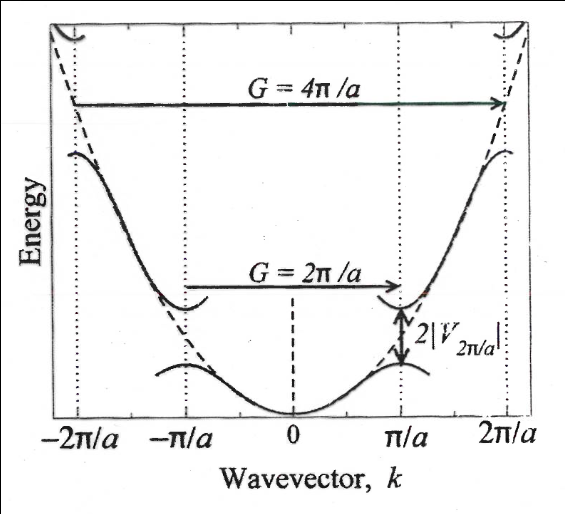
\includegraphics[scale=0.5]{disp.png}
\end{figure}
Around 0, $\pm\frac{2\pi}{a}$, it is quadratic in $k$; around $\pm\frac{\pi}{a}$, it is quadratic in $\delta$.

The figure below shows the same dispersion curves, but this time in the repeated zone scheme:
\begin{figure}[H]
    \centering
    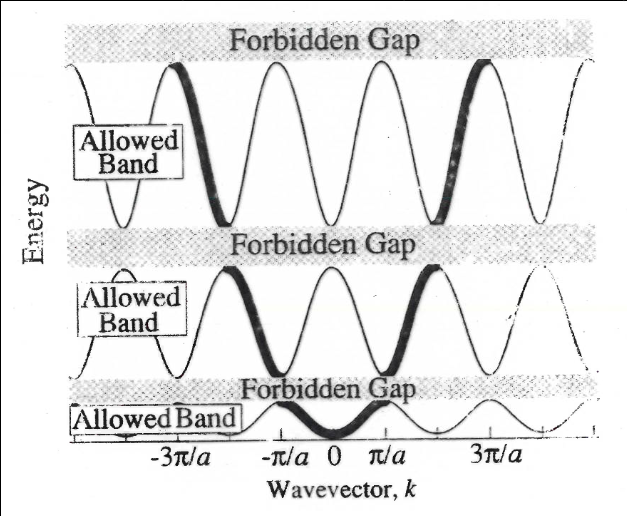
\includegraphics[scale=0.5]{rep.png}
\end{figure}
Small gaps open up at the Brillouin zone boundaries in an otherwise parabolic spectrum.
We can describe the curvature around the bottom of a band in terms of an effective mass.
We can write the dispersion to be
\begin{align}
    E_+(G+\delta) &= c_+ + \frac{\hbar^2\delta^2}{2m_+^*} \\
    E_-(G+\delta) &= c_- - \frac{\hbar^2\delta^2}{2m_-^*}
\end{align}
where $c_+$ and $c_-$ are constants.
The effective masses are then given by
\begin{equation}
    m_{\pm}^* = \frac{m}{1 \pm \frac{\hbar^2(n\pi/a)^2}{m}\frac{1}{|V_G|}}
\end{equation}
Near the bottom of a conduction band ($k = k_{min}$), the energy is given by
\begin{equation}
    E = E_{min} + \alpha|k-k_{min}|^2 + \cdots
\end{equation}
with $\alpha > 0$.
We can then define the effective mass in terms of the band curvature,
\begin{equation}
    \frac{\hbar^2}{m^*} = \frac{\p^2E}{\p k^2} = 2\alpha.
\end{equation}
Correspondingly, the group velocity is given by
\begin{equation}
    v = \frac{\del_k E}{\hbar} = \frac{\hbar(k-k_{min})}{m^*}.
\end{equation}
This definition is analogous to free electrons, 
\begin{align}
    E &= \frac{\hbar^2|k|^2}{2m} \\
    v &= \frac{\del_kE}{\hbar} = \frac{\hbar k}{m}
\end{align}
And for holes close to the top of the valence band,
\begin{equation}
    E = E_{max} - \alpha|k-k_{max}|^2 + \cdots
\end{equation}
with $\alpha > 0$.
\begin{align}
    \frac{\hbar^2}{m^*_{hole}} &= -\frac{\p^2 E}{\p k^2} = 2m \\
    E_{hole} &= c_{hole} + \frac{\hbar^2|k-k_{max}|^2}{2m^*_{hole}}
\end{align}

\section{Bloch Functions and Bloch's Theorem}
In the nearly-free electron model, we started with plane waves that were weakly perturbed by a periodic potential.
But what if in real materials, the scattering from ion cores is very strong?
Can we still use plane waves?
\textbf{Yes.}
But the plane-wave momentum is not a conserved quantity - it is the crystal momentum that is conserved.
Felix Bloch proved that the solutions of the Schrodinger equation for a periodic potential must be of the special form,
\begin{equation}
    \psi_k(r) = u_k(r)\e^{ik\cdot r}.
\end{equation}
The periodic function $u$ is a \textbf{Bloch function} and $\psi$ is a \textbf{modified plane wave.}
Because $u$ is periodic, it can be rewritten as a sum over reciprocal lattice vectors, 
\begin{equation}
    u_k(r) = \sum_G u_{G,k}e^{iG\cdot r}.
\end{equation}
This form guarantees that $u_k(r) = u_k(r+T)$ for any lattice vector $T$.
Therefore, the full wavefunction is
\begin{equation} 
    \psi_k(r) = \sum_G u_{G,k}e^{i(G+k)\cdot r}.
\end{equation}
This is an equivalent statement of Bloch's theorem.
We can write each eigenstate as being made up of a sum of plane-wave states $k$ which differ by reciprocal lattice vectors $G$.

The scattering matrix elements $\langle k'|V|k\rangle$ are zero unless $k'$ and $k$ differ by a reciprocal lattice condition - \textbf{The Laue Condition.}

The Schrodinger equation is a "block diagonal" in the space of $k$ and any eigenfunction is a mix of $k$ planewaves that differ by $G$.
One way to see this is to take the Schrodinger equation, 
\begin{equation}
    \left[\frac{p^2}{2m} + V(r)\right]\psi(r) = E\psi(r),
\end{equation}
and Fourier tranform it:
\begin{equation}
    \sum_G V_G V_{k-G} = \left[E - \frac{\hbar^2|k|^2}{2m}\right]\psi_k
\end{equation}
where we have used the fact that $V_{k-k'} \neq 0$ if $k-k' = G$.

The wave equation of an electron in a crystal is
\begin{equation}
    \Ham\psi = \e\psi
\end{equation}
or explicitly,
\begin{align}
    \left(\frac{p^2}{2m} + U(x)\right)\psi(x) = \left(\frac{p^2}{2m} + \sum_G U_Ge^{iGx}\right) \psi(x) = \e\psi(x)
\end{align}
This is written in the one electron approximation in which the orbital $\psi(x)$ describes the motion of one electron in the potential of the ion cores and in the average of the other conduction electrons.
The wavefunction $\psi(x)$ may be expressed as a Fourier series,
\begin{equation}
    \psi = \sum_k c(k)e^{ikx}
\end{equation}
where $c$ is a constant and $k$ is real.
The set of values of $k$ is $\frac{2\pi n}{L}$.

To solve the wave equation, we substitute the (3.25) into (3.24) to obtain a set of linear algebraic equations for the Fourier coefficients.
The kinetic energy term is
\begin{align}
    \frac{p^2}{2m}\psi(x) &= \frac{1}{2m}\left(-i\hbar\frac{d}{dx}\right)^2\psi(x) \\
    \implies -\frac{\hbar^2}{2m}\frac{d^2\psi}{dx^2} &= \frac{\hbar^2}{2m} \sum_k k^2c(k)e^{ikx}
\end{align}
and the potential energy term is 
\begin{equation}
    \left(\sum_G U_ge^{iGx}\right)\psi(x) = \sum_G\sum_k U_gc(k)e^{ikx}
\end{equation}
The wave equation is obtained as the sum
\begin{equation}
    \sum_k \frac{\hbar^2}{2m}c(k)e^{ikx} + \sum_G\sum_k U_Gc(k)e^{i(k+G)x} = \e\sum_k c(k)e^{ikx}
\end{equation}
Each Fourier component must have the same coefficient on both sides of the equation, which generates \textbf{the central equation,}
\begin{equation}
    (\lambda_k - \e)c(k) + \sum_G U_gc(k-G) = 0, \lambda_k = \frac{\hbar^2 k^2}{2m}.
\end{equation}
The central equation is a form the wave equation in a periodic lattice, but it emplots algebraic equations rather than differential equations.
Although this formulation looks unfamiliar and unpleasant (in principle there are an infinite number of $c(k-G)$ to be determined), in practice, a small number (2 to 4) is often enough. 

\section{An alternative and final proof of Bloch's Theorem}
Once we determined the $c$'s from 
\begin{equation}
    \psi_k(x) = \sum_G c(k-G)e^{i(k-G)x}
\end{equation}
which can be re-arranged as 
\begin{align}
    \psi_k(x) &= \left(\sum_G c(k-G)e^{-iGx}\right)e^{ikx} \\
              &= e^{ikx}U_k(x)
\end{align}
which uses the definition
\begin{equation}
    U_k(x) = \sum_G c(k-G)e^{-iGx}
\end{equation}
Because $U_k(x)$ is a Fourier series over the reciprocal lattice vectors, it is invariant under $T$, so that $U_k(x0 = U_k(x+T)$. 
We can verify this:
\begin{align}
    U_k(x+T) = \sum c(k-G)e^{-iG(x+T)} &= e^{-iGT}\left[\sum c(k-G)e^{-iGx}\right] \\
                                       &= e^{-iGT}U_k(x)
\end{align}
As $e^{-iGT} = 1$, then,
\begin{equation}
    U_k(x+T) = U_k(x)
\end{equation}

\section{Velocity of Bloch Electrons}
Our Bloch electrons in energy bands travel through the lattice as travelling waves with a group velocity given by
\begin{equation}
    v_g = \frac{d\om}{dk}.
\end{equation}
As $E = \hbar\om$, then
\begin{equation}
    v_g = \frac{1}{\hbar}\frac{dE(k)}{dk}.
\end{equation}
But what about the electrons at the bottom of the energy band in the nearly-free electron model? 
Has their velocity changed?
\begin{align}
    v_g &= \frac{1}{\hbar}\frac{dE(k)}{dk}, E = \frac{\hbar^2k^2}{2m_e} \\
    v_g &= \frac{1}{\hbar}\frac{d}{dk}\left[\frac{\hbar^2k^2}{2m}\right] = \frac{\hbar k}{m_e} = \frac{p}{m_e} = v
\end{align}
where $p$ is the crystal momentum of the Bloch electrons.

\section{Current carried by energy bands}
Once we know the velocity of an electron in a band, we can determine the current carried by a collection of electrons in an energy band. 
The current density is given by $j = ne\langle v\rangle$ where $\langle v\rangle$ is the average velocity of the electrons in the band.

Suppose we have $M$ states in a filled band occupied by $2M$ electrons, 
\begin{equation}
    \langle v\rangle = \frac{1}{\hbar} \int_{k = -\pi/a}^{k=+\pi/a} \frac{dE}{dk}\frac{dk}{2\pi}
\end{equation}
or 
\begin{equation}
    \langle v\rangle = \frac{1}{2\pi\hbar} \left[E\left(\frac{\pi}{a}\right) - E\left(-\frac{\pi}{a}\right)\right]
\end{equation}
But as found earlier, $k = \pm \frac{\pi}{a}$ are physically equivalent values of the Bloch wavevector.
So $E\left(\frac{\pi}{a}\right) = E\left(-\frac{\pi}{a}\right)$ and $\langle v\rangle = 0$.
If $\langle v\rangle = 0$, then $j = 0$.

A completely filled energy band makes no contribution to the current carried by a crystal.

\chapter{}
\section{Successes and Failures of the Band Structure Picture of Metals and Insulators}
Successes:
\begin{itemize}
    \item The most complete description of condensed matter we have.
    \item Using just the number of electrons, it can predict metals, semimetals, insulators, semiconductors (doped, undoped).
\end{itemize}
Failures:
\begin{itemize}
    \item The model is based on the one electron approximation. 
    \item All failures are due to strong electron-electron interactions. 
    \item A new theory is being developed.
    \item Two major classes of materials cannot be explained using bandstructure models:
        \begin{enumerate}
            \item Transition Metal Oxides:
                \begin{itemize}
                    \item Transition metal oxides like $CoO$, $NiO$ have half-filled bands but are insulators. 
                    \item Doping can produce superconductors $La_{2-x}SP_x CuO_4$.
                    \item Oxides can display metal-insulator transitions. 
                \end{itemize}
            \item Magnets and Magnetisms
                \begin{itemize}
                    \item Magnetic spins have strong interactions. 
                    \item Many different magnetic interactions, structures, properties.
                \end{itemize}
        \end{enumerate}
\end{itemize}

\section{Magnetic fields and magnetic materials}
Let us first define some terms:
\begin{itemize}
    \item $\B$ is the magnetic flux density, or magnetic induction
    \item $\He$ is the magnetic field strength
\end{itemize}
In free space (vacuum), there is no magnetisation. 
The magnetic field can be described by the vector fields $\B$ and $\He$ which are linearly related by 
\begin{equation}
    \B = \mu_0 \He
\end{equation}
where $\mu_0 = 4\pi\times10^{-7}\,\text{H m}^{-1}$ is the magnetic permeability of free space.

The two magnetic fields $\B$ and $\He$ are just caled versions of each other, the former measured in Tesla (T), and the latter measured in A m$^{-1}$.
The magnetic flux density of a magnetic material is then 
\begin{equation}
    \B = \mu \He
\end{equation}
where $\mu$ is the magnetic permeability. 

\section{Magnetic moments and Magnetisation}
\subsection{The Classical Model - A review of Electromagnetism}
\begin{wrapfigure}{r}{0.4\textwidth}
    \centering
    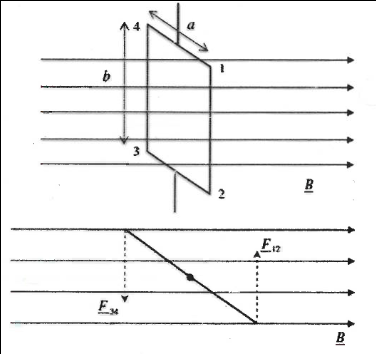
\includegraphics[width=0.35\textwidth]{induct.png}
\end{wrapfigure}
Let us start by considering a current, $I$, running through a rectangular loop of wire suspended on two sides. 
The metallic loop is placed in the presence of a magnetic induction, $\B$, directed perpendicular to the axis of suspension, around which the coil is free to rotate. 
The force on the side 1-2 will be $F_{12} = I\unl{b}\times\B$ where $\unl{B}$ is the 'vector length' of 1-2 (or 3-4). 
Similarly, $F_{14} = I\unl{a}\times\B$.
Now $F_{12} = -F_{34}$ and $F_{14} = -F_{23}$ so there is no net force on the loop, but $F_{12}$ and $F_{34}$ produce a torque, $\tau = I\unl{s}\times\B$ where $\unl{s}$ is the area vector ($|\unl{s}|$ is the area of the loop).

We define the magnetic moment of the current loop as
\begin{equation}
    \unl{m} = I\unl{s}
\end{equation}
with units of A m$^2$.
Hence the torque on the magnetic moment is 
\begin{equation}
    \tau = \unl{m} \times \B
\end{equation}
Thus the effect of $\B$ is to rotate $\unl{m}$ until it is parallel to the magnetic induction. 
Assuming there are no frictional forces, the work done by the turning force will be conserved, which gives the expression for the energy of a magnetic moment in the presence of a magnetic induction, 
\begin{equation}
    E = 0\mu\cdot\B.
\end{equation}

For the simple case of an electron orbiting a nucleus (Bohr atom) with velocity $\unl{v}$ with a circular orbit of radius $\unl{r}$,
\begin{align}
    |m| = I|s| &= \frac{e\unl{v}}{2\pi \unl{r}} \cdot \pi r^2 \\
               &= \frac{e\unl{v}}{2}\cdot\unl{r}
\end{align}
The orbital angular momentum $\unl{G}$ is 
\begin{equation}
    \unl{G} = m_e(\unl{r}\times \unl{v})
\end{equation}
giving the magnetic moment
\begin{equation}
    \unl{m} = \frac{-|e|\unl{G}}{2m_e}
\end{equation}
and the magnetic moment of a multi-electron Bohr atom to be the sum of the magnetic moments of each electron, i.e.
\begin{equation}
    \unl{m}_{atom} = \sum_i \unl{m}_i = -\frac{|e|}{2m_e}\sum_i \unl{G}_i
\end{equation}
Therefore, from $\tau = \unl{m}\times\B$, we would expect a solid containing atoms, each of magnetic moment $\unl{m}$ to respond to the presence of a magnetic induction. 
\begin{figure}[H]
    \centering
    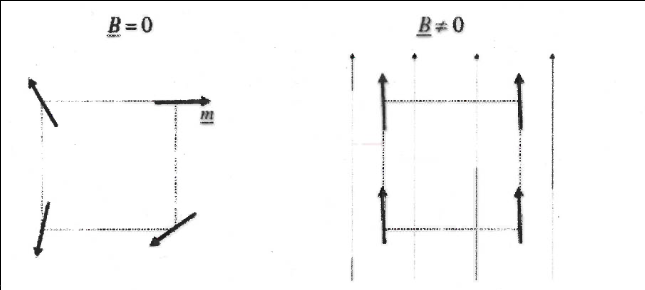
\includegraphics[scale=0.5]{torque.png}
\end{figure}
We can define the total magnetisation, $\unl{M}$ of the magnetic moments of $N_A$ atoms per unit volume, $V$,
\begin{equation}
    \unl{M} = \frac{\unl{m}N_A}{V}
\end{equation}
We can infer the relation between the magnetisation $\unl{M}$ and the magnetic field (or magnetic flux density) $\B$ if we consider a solid filled with many small elementary closed current loops (magnetic moment). 
The neighbouring currents cancel so that only the surface currents remain uncompensated. 
Assuming there are $n$ current laters per unit length along the direction of magnetisatino and the area of each loop is $s$ (current $I$), there are $\frac{I}{s}$ loops per unit volume of the magnetic material, 
\begin{equation}
    |M| = \frac{n}{s}(Is) = nI
\end{equation}
I.e. the magnetisation acts as a magnetic field which adds to the applied magnetic field.
Thus the magnetic induction is
\begin{equation}
    \B = \mu_0(\He+\unl{M})
\end{equation}

\section{A Cautionary Tale: Classical Mechanics and Magnetic Moments}
During this course, we will seek insight into our derived equations using classical mechanics and EM, but magnetism is inherently a quantum phenomena. 
So here is a cautionary tale from Niels Bohr. 

\subsection{Canonical Momentum}
In classical mechanics, the force $F$ on a particle with charge $q$ with velocity $v$ in an electric field $\e$ and magnetic field $\B$ is the Lorentz force. 
\begin{equation}
    \unl{F} = q(\e + \unl{v}\times\B)
\end{equation}
This modifies the momentum of a charged particle in a magnetic field.
Using $F = m\frac{dv}{dt}$, $\B = \del\times\unl{A}$, and $\e = -\del V - \frac{\p A}{\p t}$, where $V$ is the electric potential, $\unl{A}$ is the magnetic vector potential and $m$ is the mass of the particle. 
\begin{equation}
    m\frac{dv}{dt} = -q\del V - q\frac{\p \unl{A}}{\p t} + q\unl{v} \times (\del\times\unl{A})
\end{equation}
The vector identity
\begin{equation}
    \unl{v}\times(\del\times\unl{A}) = \del(\unl{v}\cdot\unl{A}) - (\unl{v}\cdot\del)\unl{A}
\end{equation}
can be used to simplify this. 
\begin{equation}
    m\frac{dv}{dt} + q\left(\frac{\p\unl{A}}{\p t} + (\unl{v}\cdot\del)\unl{A}\right) = -q\del(V - \unl{v}\cdot\unl{A})
\end{equation}
This can be rewritten as
\begin{equation}
    \frac{d}{dt}(m\unl{v} + q\unl{A}) = -q\del(V - \unl{v}\cdot\unl{A})
\end{equation}
where $\frac{d\unl{A}}{dt}$ is the convective derivative of $\unl{A}$
\begin{equation}
    \frac{d\unl{A}}{dt} = \frac{\p \unl{A}}{\p t} + (\unl{v}\cdot\del)\unl{A}
\end{equation}
which measures the rate of change of $A$ at the location of the moving particle. 
Eqn (4.12) is like Newton's Second Law. 
This allows us to define a \textbf{canonical momentum},
\begin{equation}
    \unl{p} = m\unl{v} + q\unl{A}.
\end{equation}
Note that  if $\unl{A} = 0$, then $\unl{p} = m\unl{v}$.

\section{The Bohr-van Leeuwen Theorem}
The next step is to calculate the net magnetic moment of a system of electrons in a solid.
This is the magnetisation, the magnetic moment per unit volume, that is induced by the magnetic field. 

\begin{wrapfigure}{r}{0.3\textwidth}
    \centering
    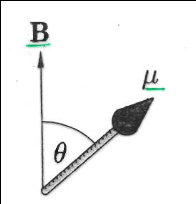
\includegraphics[scale=0.4]{magnet.png}
\end{wrapfigure}
Consider a magnetic moment $\mu$ in a magnetic field $\B$. 
The energy $E$ of the magnetic moment is given by
\begin{equation}
    E = -\mu\cdot\B = -\mu\B\cos\theta
\end{equation}
so that the energy is minimised when the magnetic moment lies along the magnetic field. 
Thus the magnetisation is proportional to the rate of change of energy of the system with applied magnetic field. 
Now the Lorentz Force shows that the effect of a magnetic field is always to produce forces on charged particles which are perpendicular to their velocities. 
Thus no work is done and therefore the energy of a system cannot depend on the applied magnetic field. 
If the energy of the system does not depend on the applied magnetic field, then there can be no magnetisation.

This idea is enshrined in the Bohr-van Leeuwen theorem which states that in a classical system, there is no thermal equilibrium magnetisation. 
In classical statistical mechanics, the partition function $Z$ for $N$ particles, each with charge $q$ is proportional to
\begin{equation}
    \iint \cdots \int \exp\left(\frac{-E}{k_BT}\{r_i,p_i\}\right) d\unl{r}_1\cdots d\unl{r}_N\; d\unl{p}_1\cdots d\unl{p}_N
\end{equation}
Here $E(\{r_i,p_i\})$ is the energy associated with the $N$ charged particles having positions $r_1,r_2,\cdots,r_N$ and momenta $p_1,p_2,\cdots,p_N$.
The integral is over $6N$ dimensional phase space.
The effect of a magnetic field is to shift the momenta of each particle by an amount $q\unl{A}$. 
We must therefore replace $\unl{p}_i$ with $\unl{p}_i-q\unl{A}$.
The limits of the momentum integrals are $\pm\infty$ so the shift is simply a shifting of the origin of the momentum integrations. 
Hence the partition function is not a function of magnetic field, so neither is the free energy,
\begin{equation}
    F = -k_BT\ln(Z).
\end{equation}
Thus the magnetisation must be zero in a classical system. 
This result seems surprising. 
With no applied magnetic field, electrons go in straight lines; but with magnetic fields, their paths are curved (helical). 
The figure shows the curved cylotron orbits, all curved in the same sense. 
Do these contribute a net magnetic moment?
\begin{figure}[H]
    \centering
    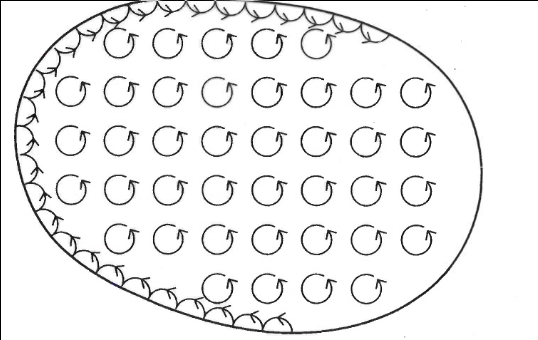
\includegraphics[scale=0.5]{cyclo.png}
\end{figure}
No!
Because there are precisely cancelled out by the large clockwise current associated with the surface currents. 
The Bohr-Leeuwen theorem is correct, but clearly at odds with experimental observations. 
The assumption of classical mechanics is wrong. 
Classical mechanics is insufficient to explain this most basic \textbf{quantum} property. 
We conclude that we cannot avoid using quantum machanics to explain magnetic behaviour. 

\chapter{}
\section{Magnetic Materials}
Magnetism is a quantum mechanical effect as a strictly classical system in thermal equilibrium can display no magnetic moment. 
Even in the presence of a magnetic field. 
The magnetic moment of a free atom has three principle sources
\begin{enumerate}
    \item the spin of the electrons 
    \item their orbital angular momentum about the nucleus
    \item the change in the orbital moment induced by an applied magnetic field
\end{enumerate}

\section{Magnetic Measurements}
What magnetic measurements can we perform to measure the magnetic properties of magnetic materials?
We can measure the change in voltage produced in a coil of $N$ wire turns of cross-sectional area $A$ when the magnetic flux changes when a sample is places in a high magnetic field,
\begin{equation}
    V = -NA\frac{d\B}{dt}
\end{equation}
This is the induction method for measuring magnetisation. 
But this method has high errors due to design of pick-up coils, magnetic images etc. 

A far more precise induction method is the vibrating sample magnetometer. 
The sample is vibrated at $90^\circ$ to the magnets at a fixed frequency producing an alternating inductive signal.
Spurious vibrations at the frequency are avoided by a reference signal.

\section{Magnetic Susceptibility}
The magnetic susceptibility is a proportionality constant that indicates the degree of magnetisation of a material in response to an applied magnetic field. 
The volume susceptibility $\chi_V$ is
\begin{equation}
    \unl{M} = \chi_V\unl{H}
\end{equation}
where $\unl{M}$ is the magnetisation of the material and $\unl{H}$ is the magnetic field strength. 
The mass susceptibility $\chi_m$ (units of $\text{m}^3\,\text{kg}^{-1}$) is
\begin{equation}
    \chi_m = \frac{\chi_V}{\rho}
\end{equation}
where $\rho$ is the density.
The molar susceptibility $\chi_{mol}$ (units of $\text{m}^3\,\text{mol}^{-1}$)
\begin{equation}
    \chi_{mol} = M\chi_m = \frac{M\chi_V}{\rho}
\end{equation}
The magnetic induction $\B$ is related to $\unl{H}$ by
\begin{align}
    \B &= \mu_0(\unl{H}+\unl{M}) = \mu_0(1+\chi_V)\unl{H} \\
       &= \mu\unl{H}
\end{align}
where $\mu_0$ is the magnetic constant of vacuum permeability ($4\pi\times10^{-7}\,\text{H m}^{-1}$) and $(1+\chi_V)$ is the relative permeability of the material.
We can thus relate the vilume magnetic susceptibility $\chi_V$ to the magnetic permeability $\mu$
\begin{equation}
    \mu = \mu_0(1+\chi_V)
\end{equation}

\section{Magnetic Susceptibility Measurements}
Volume magnetic susceptibility measurements can be undertaken by measuring the force change felt upon the application of a magnetic field gradient. 
Early measurements hung a sample between magnetic pole pieces. 
When the electromagnet was turned off, the change in weight was proportional to the magnetic susceptibility. 

Nowadays, Evan's balances measure the force change on a strong compact magnet upon insertion of the sample, calibrated with known standards.
Two pairs of magnets are placed at opposite ends of a beam making a balanced system. 
When a sample is introduced into the field of one magnet, that magnet experiences a force that deflects the beam.
\begin{figure}[H]
    \centering
    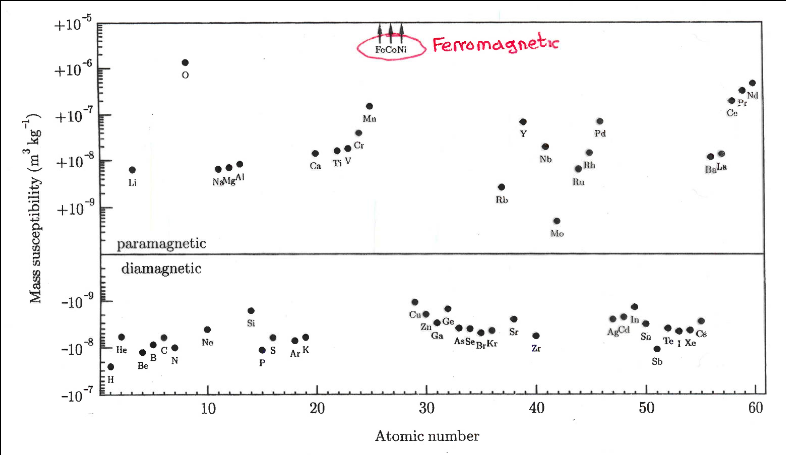
\includegraphics[scale=0.5]{mags.png}
\end{figure}

\begin{itemize}
    \item \textbf{Ferromagnets} display very high, positive magnetic susceptibility. 
        They display a spontaneous magnetic field even in the absence of an applied magnetic field. 
    \item \textbf{Paramagnets}. Most materials are paramagnetic.
        Positive, but small magnetic susceptibility. 
    \item \textbf{Diamagnetism} occurs in all materials, often masked. 
        Small negative $\chi$, temperature independent.
    \item \textbf{Antiferromagnetism} - positive magnetic susceptibility, complex temperature dependence.
        At high $T$, often paramagnetic.
        $\chi$ reaches a maximum at Neel temperature, below which they are antiferromagnetic.
\end{itemize}

\begin{figure}[H]
    \centering
    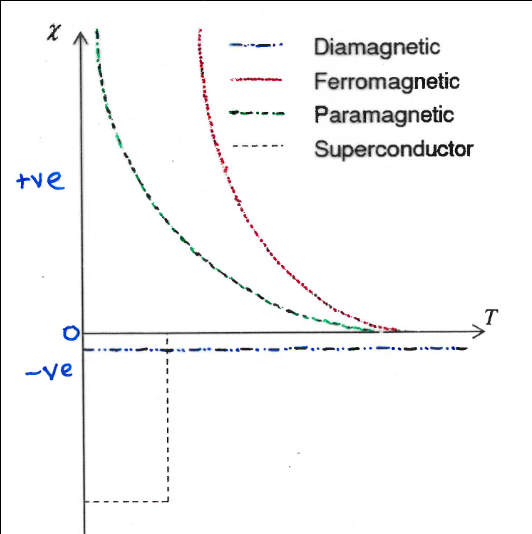
\includegraphics[scale=0.4]{dia.png}
    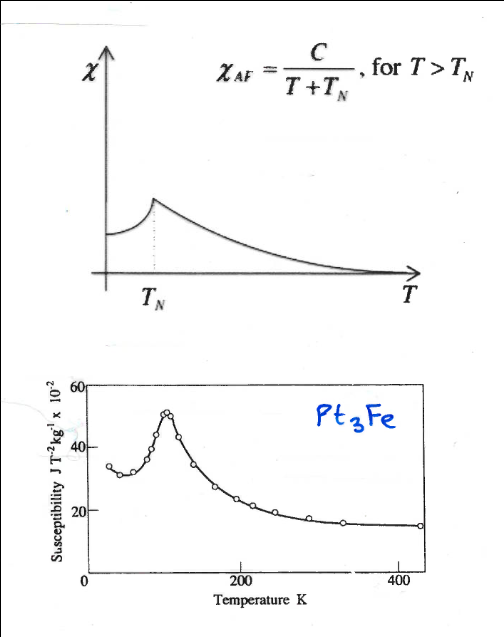
\includegraphics[scale=0.35]{anti.png}
\end{figure}

\chapter{Diamagnetism}
Diamagnetism is present in all matter, but often masked by paramagnetism or ferromagnetism. 
Diamagnetic materials display a temperature-independent negative magnetic susceptibility. 
Diamagnetism does not require the atoms to have a non-zero magnetic moment in the absence of a magnetic field. 
It is associated with the tendency of electrical charges to partially shield the interior from an applied magnetic field. 
It is very similar to Lenz's law: \emph{when the flux through an electrical circuit is changed, an induced current is set up to oppose the flux change.}

We will start by following Langevin's classical approach to understanding the origin of diamagnetism.
We start by recalling the magnetic moment of a simply Bohr atom, with an electron orbiting a nucleus with radius $\vr$ and tangential velocity, $\vec{v}$.
\begin{equation}
    \unl{m} = \frac{-|e|\unl{G}}{2m_e}
\end{equation}
We now apply a magnetic field $\B$ normal to the electron orbit, which generates an electric field $\E$ which produces a force on the orbital electron. 
This accelerates, or decelerates the orbital motion, changing the orbital velocity and hence the magnetic moment in such a way to oppose the applied magnetic field. 
Integrating the Maxwell-Faraday equation over the area of the circular orbit, 
\begin{align}
    -\int \frac{\p\B}{\p t}\cdot dA &= \int (\del\times\E)\cdot dA = \oint \E\cdot dl \\
    -\left(\frac{\p\B}{\p t}\right)\pi r^2 &= 2\pi r\E.
\end{align}
The tangential electric field, 
\begin{equation}
    \E = -\left(\frac{\p\B}{\p t}\right)\frac{r}{2},
\end{equation}
produces a torque,
\begin{equation}
    \vr\times\vec{F} = -|e|\E\vr,
\end{equation}
parallel to $\B$ which changes the angular momentum $\unl{G}$ such that
\begin{equation}
    \vr\times\vec{F} = \frac{\p\unl{G}}{\p t} = |e|\left(\frac{\p\B}{\p t}\right)\frac{r^2}{2}
\end{equation}
Integrating over the time to turn on the magnetic field gives the additional angular momentum
\begin{equation}
    \Delta G = |e|r^2\frac{\B}{2}
\end{equation}
parallel to $\B$, which describes a field-induced magnetic moment directed opposite to $\B$ of
\begin{equation}
    \Delta m = \frac{-|e|\Delta G}{2m_e} = -\frac{e^2r^2\B}{4m_e}.
\end{equation}
This result only applied when $\B$ is perpendicular to the electron motion. 
If $\B$ were parallel, then $\Delta m = 0$.
Averaging over all possible orientations gives
\begin{align}
    \Delta m &= \frac{-e^2\langle r^2\rangle\B}{4m_e} = \frac{-e^2\B}{4m_e}\left(\frac23\langle r^2\rangle\right) \\
             &= -\frac{e^2\langle r^2\rangle\B}{6m_e} 
\end{align}
If there are $N$ atoms per unit volume, 
\begin{equation}
    \chi_d = \frac{\mu}{H} = \frac{\mu_0N\Delta m}{\B} = -\frac{\mu_0Ne^2}{6m_e}\langle r^2\rangle
\end{equation}
For atoms with atomic number $Z$,
\begin{equation}
    \chi_d = -\frac{\mu_0NZe^2}{6m_e}\langle r^2\rangle
\end{equation}
But is this classical prediction correct?
Let us check by using a quantum mechanics approach. 
The momentum $\vp$ can be defined by the Lagrangian
\begin{equation}
    \vp \equiv \frac{\p L}{\p \unl{\dot{q}}} = M\unl{\dot{q}} + \frac{Q}{c}A
\end{equation}
and the Hamiltonian is
\begin{align}
    \Ham(\vp\cdot\unl{q}) &\equiv \vp\cdot\unl{\dot{q}} - L \\
    \Ham &= M\dot{q}^2 + \frac{Q}{c}\dot{q}\cdot R - \frac12M\dot{q}^2 + Q\psi = \frac{Q}{c}\dot{q}\cdot A \\
         &= \frac{1}{2M}(\vp - \frac{Q}{c}A)^2 + Q\psi
\end{align}
The effect of a magnetic field is to add to the Hamiltonian the terms
\begin{equation}
    \Ham = \frac{ie\hbar}{2mc}\left(\del\cdot A + A\cdot\del\right) + \frac{e^2}{2mc}A^2
\end{equation}
For an electron these terms are a small perturbation. 
If the magnetic field is uniform and in the $z$-direction
\begin{align}
    A_x &= -\frac12 y\B & A_y &= \frac12 x\B & A_z &= 0 
\end{align}
and then
\begin{align}
    \Ham &= \frac{ie\hbar\B}{2mc}\left(x\frac{\p}{\p y} - y\frac{\p}{\p x}\right) + \frac{e^2\B^2}{8mc^2}(x^2+y^2) 
\end{align}
The first term is proportional to the orbital angular momentum component $L_2$ - only paramagnetism. 
The second term gives for a spherical symmetric system, 
\begin{equation}
    E' = \frac{e^2\B^2}{12mc^2}\langle r^2\rangle
\end{equation}
by first order perturbation theory. 
The associated magnetic moment is diamagnetic. 
\begin{equation}
    \mu = -\frac{\p E'}{\p\B} = -\frac{e^2\langle r^2\rangle}{6m_e}\B
\end{equation}
This is in agreement with the classical result. 

So far, we have used only first order perturbation theory. 
As $T$ is increased, magnetic states above the ground state become more important, but a very small effect.
\begin{figure}[H]
    \centering
    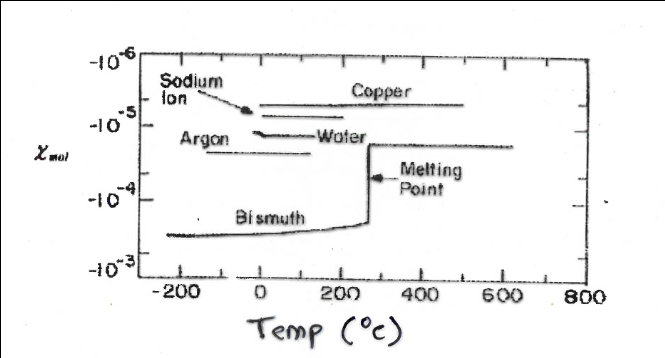
\includegraphics[scale=0.5]{bismuth.png}
\end{figure}
Diamagnetic susceptibilities are usually temperature-independent.
What about Bismuth?

We can this $\mu$ by plotting $\chi_{mol}$ vs $Z_{eff}r^2$ where $Z_{eff}$ is the number of electrons in the outer shell of an ion and $r$ is the measure ionic radius.
\begin{equation}
    \sum_{i=1}^{Z_{eff}} \langle r_i^2\rangle \approx Z_{eff}r^2
\end{equation}
Results for various ions are shown below, and the graph is indeed linear. 
\begin{figure}[H]
    \centering
    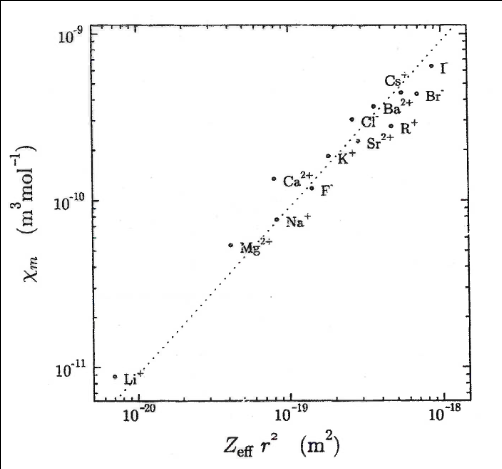
\includegraphics[scale=0.5]{ions.png}
\end{figure}
As diamagnetic materials have a magnetic susceptibility that is negative, this means they have internal magnetic fields that are oppositely directed to applied magnetic fields. 
This means that diamagnetic materials can be moved (repelled) by application of high magnetic fields. 

\chapter{}
\section{Paramagnetism}
Paramagnetism corresponds to materials with a positive susceptibility so that an applied magnetic field induces a magnetisation that aligns parallel. 
Diamagnetism considered atoms or molecules with no unpaired electrons. 
Here we will consider mateirals with unpaired electrons and non-zero magnetic moment. 

Without an applied magnetic field, these moments point in random directions because of very weak interaction with neighbouring moments.
Applications of a magnetic field will tend to align up the moments, temperature will increase entropy, and randomise them. 
The magnetic moment of an atom or ion in free space is 
\begin{equation}
    \mu = \gamma\hbar\unl{J} = -g\mu_B\unl{J}
\end{equation}
where $\unl{J}$ (total angular momentum) is the sum of the orbital momentum $\unl{L}$ and the spin angular momentum $\unl{S}$,
\begin{equation}
    \unl{J} = \unl{L} + \unl{S}.
\end{equation}
These are all measured in units of $\hbar$.

In this section, we will assume that each atom has a magnetic moment of $\mu$.
The constant $\gamma$ is the ratio of the magnetic moment to the angular momentum is the gyromagnetic constant,
\begin{equation}
    g\mu_B \equiv -\gamma\hbar.
\end{equation}
For an electron spin, $g=2.0023$, usally taken as $2.00$.
For a free atom, the $g$ factor is given by the Lande equation:
\begin{equation}
    g = 1 + \frac{J(J+1) + S(S+1) - L(L+1)}{2J(J+1)}.
\end{equation}
The Bohr magneton, 
\begin{equation}
    \mu_B \equiv \frac{e\hbar}{2m} = 9.274\times10^{-24}\text{ J T}^{-1}
\end{equation}

\section{The Brillouin Function}
\begin{wrapfigure}{r}{0.4\textwidth}
    \centering
    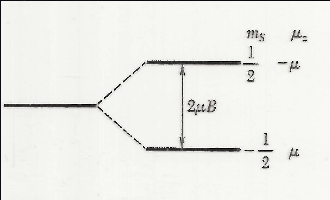
\includegraphics[width=0.4\textwidth]{mub1.png}\\
    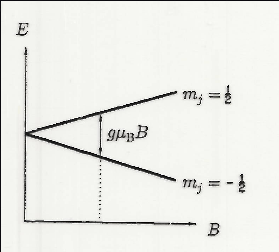
\includegraphics[width=0.4\textwidth]{mub2.png}
\end{wrapfigure}
The energy levels of an atom in an applied magnetic field $\B$ are
\begin{equation}
    u = -\unl{\mu}\cdot\B = m_jg\mu_b\B
\end{equation}
where $m_j$ is the azimuthal quantum number
\begin{equation}
    m_j = -J,-J+1,-J+2,\cdots,J-2,J-1,J.
\end{equation}
For a single quantum spin with $J = \frac12$, there are only two possible values of the z-component of the magnetic moment, $m_j = \pm\frac12$, and $g=2$.
They can be pointing either parallel to $\B$ or antiparallel to $\B$.
Thus the magnetic moments are $\pm\mu_B$.

In the general case, an atom with angular momentum $\unl{J}$ would have $2J+1$ levels in a magnetic field.
The magnetisation is given by
\begin{align}
    M &= N_gJ\mu_BB_J(y) & y &= \frac{gJ\mu_BB}{k_BT}
\end{align}
where the Brillouin function is defined by
\begin{equation}
    B_J(y) = \frac{2J+1}{2J}\coth\left(\frac{2J+1}{2J}y\right) - \frac{1}{2J}\coth\left(\frac{y}{2J}\right)
\end{equation}
For $J=\infty$ (semiclassical treatment with a continuous function and no quantised states), it reduces to a \emph{Langevin function}:
\begin{equation}
    B_\infty(y) = L(y) = \coth(y) - \frac{1}{y}
\end{equation}
Thus the ratio of the magnetisation to the emph{saturation magnetisation} is
\begin{equation}
    \frac{M}{M_S} = \frac{\langle\mu_z\rangle}{\mu} \approx \frac{y}{3} = \frac{\mu B}{3k_BT}
\end{equation}
Hence the magnetic susceptibility in low fields, 
\begin{equation}
    \chi = \frac{M}{H} \approx \frac{\mu_0M}{B} = \frac{n\mu_0\mu^2}{3k_BT} = \frac{C}{T}
\end{equation}
\begin{figure}[H]
    \centering
    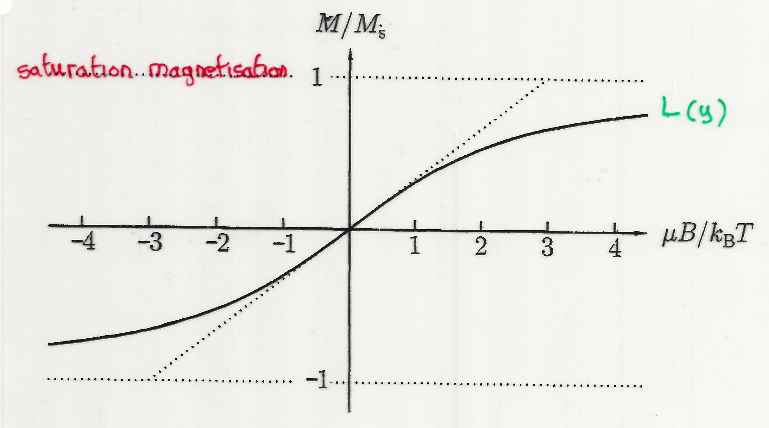
\includegraphics[scale=0.5]{satmag.png}
\end{figure}
For a quantum spin, $J = \frac12$, the Brillouin function reduces to
\begin{equation}
    B_{1/2}(y) = \tanh(y),
\end{equation}
and the ratio magnetisation/saturation magnetisation,
\begin{equation}
    \frac{M}{M_s} = \frac{\langle m_j\rangle}{J} = \tanh(y)
\end{equation}
where
\begin{equation}
    y = \frac{\mu_BB}{k_BT} = \frac{g\mu_BJB}{k_BT}
\end{equation}
Thus in small applied fields, 
\begin{equation}
    \tanh\left(\frac{\mu_B}{k_BT}\right) \approx \frac{\mu_B}{k_BT}
\end{equation}
and hence the magnetic susceptibility,
\begin{equation}
    \chi = \frac{n\mu_0\mu_B^2}{k_BT} = \frac{C}{T}
\end{equation}
\begin{figure}[H]
    \centering
    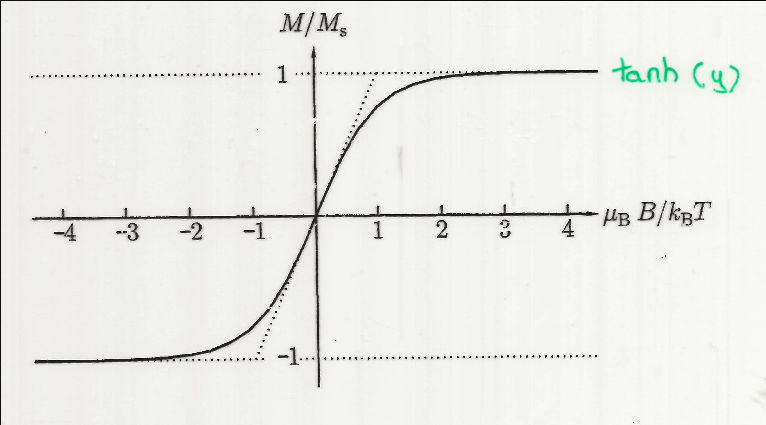
\includegraphics[scale=0.5]{tanh.png}
\end{figure}
Thus for a paramagnetic solid consisting of $n$ non-interacting spin-$\frac12$ ions per unit volume as a function of $\frac{k_BT}{\mu_BB}$.
\begin{figure}[H]
    \centering
    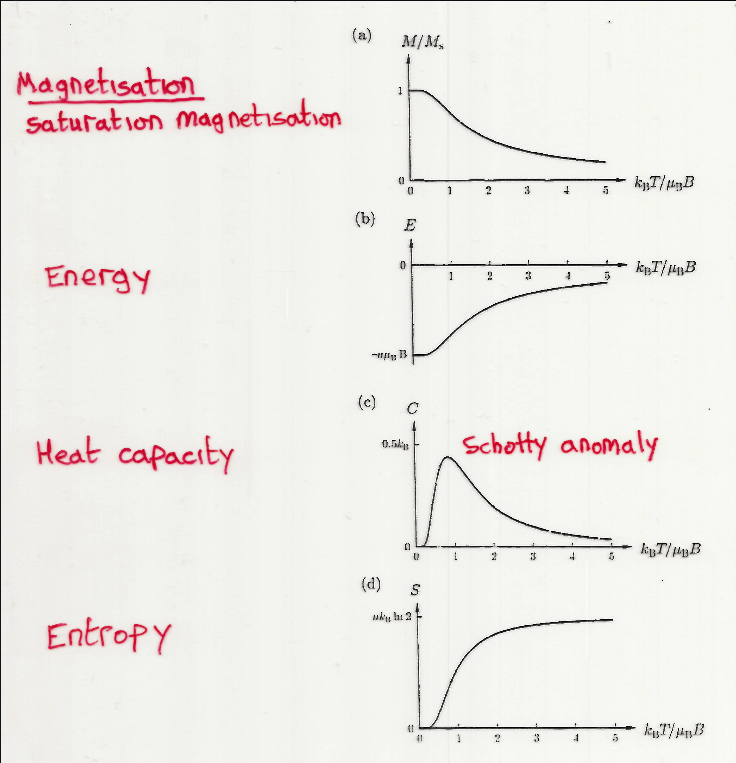
\includegraphics[scale=0.5]{func.png}
\end{figure}
Thus $J=\infty$ and $J=\frac12$ are the limits of a continuous Brillouin function.
\begin{figure}[H]
    \centering
    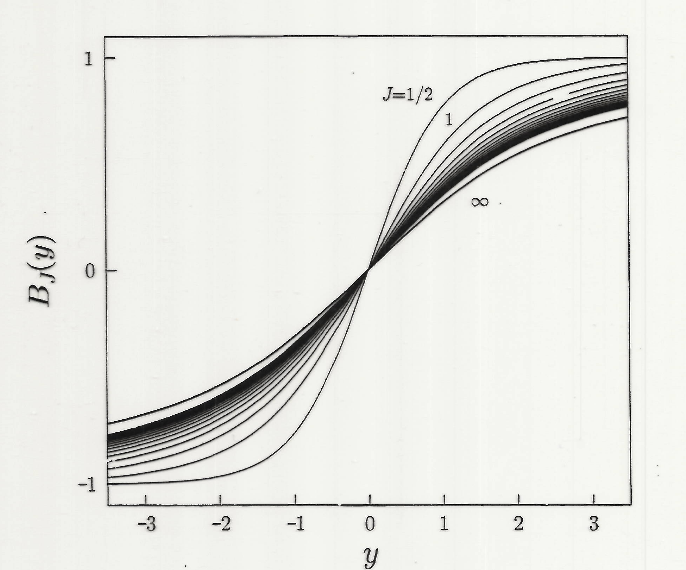
\includegraphics[scale=0.5]{lims.png}
\end{figure}
For the general case of the Brillouin function,
\begin{align}
    y &= \frac{\mu B}{k_BT} << 1 \\
    \coth(y) &= \frac{1}{y} + \frac{y}{3} - \frac{y^2}{45} \\
    \chi_p &= \frac{M}{H} \approx \frac{\mu_0M}{B} = \frac{n\mu_0\mu_{eff}^2}{3k_BT} = \frac{C}{T}
\end{align}
where $C$ is known as the \emph{Curie constant} and $\chi_p = \frac{C}{T}$ is Curie's law. 
A measurement of $\chi_p$ therefore allows us to deduce $\mu_{eff}$, the effective magnetic moment, 
\begin{equation}
    \mu_{eff} = g_j\mu_B\sqrt{J(J+1)}
\end{equation}
The Curie Lae dependence, $chi_p \propto \frac{1}{T}$:
\begin{figure}[H]
    \centering
    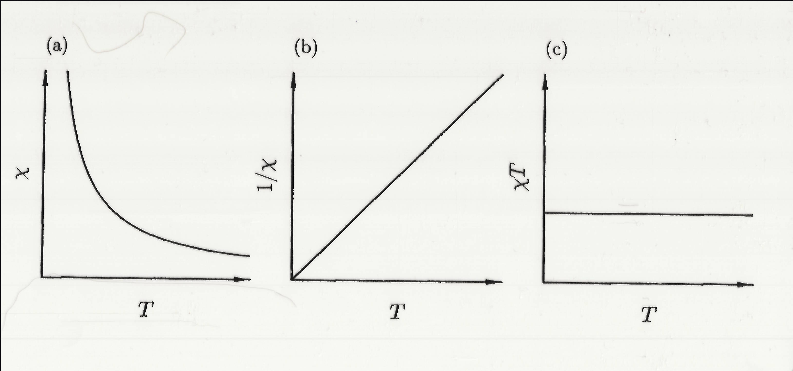
\includegraphics[scale=0.5]{curie.png}
\end{figure}

\section{Van Vleck Paramagnetism}
What happens if $J=0$?
No paramagnetic effect as
\begin{equation} 
    \langle 0|\hat{\mu}|\rangle = g_j\mu_B\langle 0|\hat{J}|0\rangle = 0
\end{equation}
But this is only correct in 1st-order perturbation theory. 
In 2nd order:
\begin{equation}
    \Delta E_0 = \sum_n \frac{|\langle 0|(L+gS)\cdot B|n\rangle|^2}{E_0-E_n} +\underbrace{\frac{e^2}{8m_e}\sum_i (B\times r_i)^2}_{\text{diamagnetism}}
\end{equation}
The first term is summed over all excited states:
\begin{equation}
    \chi = \frac{N}{V}\left(2\mu_B^2\sum_n\frac{|\langle 0|L_z + gS_z|n\rangle|^2}{E_n-E_0} - \frac{e^2\mu_0}{6m_e}\sum_{i=1}^Z \langle r_i^2\rangle\right)
\end{equation}
where the first term is positive (paramagnetic) and largely temperature independent.

\section{The Ground State of an atom/ion}
A typical atom can contain many electrons, some in unfilled shells which give non-zero spin and angular momentum. 
An atom can have total orbital angular momentum $\hbar L$, and total spin angular momentum $\hbar S$.
They can combine in $(2L+1)(2S+1)$ different ways. 
\begin{figure}[H]
    \centering
    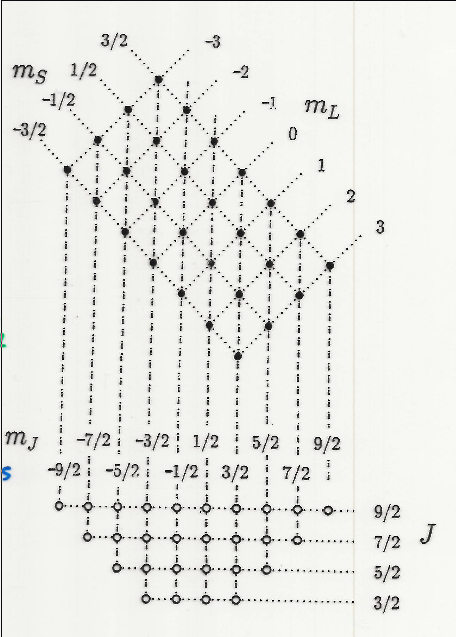
\includegraphics[scale=0.5]{combs.png}
\end{figure}
So far we have kept the spin and orbital angular momentum separate, since they are independent.
However, they do weakly couple, vie the spin-orbit interaction. 
This acts as a weak perturbation on states with well defined $\unl{L}$ and $\unl{S}$ states.
Because of this, $\unl{L}$ and $\unl{S}$ are not separately conserved (not good quantum numbers).
But the total angular momentum $\unl{J} = \unl{L}+\unl{S}$ is conserved.
The problem remains: out of so many possible combinations of angular momentum quantum numbers, how do we determine the ground state?

\section{Hund's Rules}
Hund's rules can predict the ground state configuation but do not imply anything about the ordering of the excited states. 
They also assume only one subshell is incomplete. 
They are listed in order of decreasing importance. 
\begin{enumerate}
    \item Electrons occupy available states such that the maximum total spin angular momentum is obtained without violating the Pauli exclusion principle, use
        \begin{equation}
            S = \sum m_s
        \end{equation}
    \item Electrons occupy available states such that the maximum value of the total orbital angular momentum is obtained consistent with the given value of $S$, use
        \begin{equation}
            L = \sum m_L
        \end{equation}
    \item The total atomic angular momentum $J$ is given by:
        \begin{itemize}
            \item $J = |L-S|$ when the shell is less than half full
            \item $J = |L+S|$ when the shell is greater than half full
            \item $J=S$ when the shell is exactly half full, i.e. $L=0$
        \end{itemize}
\end{enumerate}
Hund's rules minimise energy. 
\begin{itemize}
    \item The first rule minimises Coulomb energy by Pauli exclusion principle - reduces Coulomb repulsion
    \item The second rule minimises energy.
        Imagine electrons in orbits rotating in the same direction - avoids repulsion.
    \item The third rule minimises the spin-orbit energy.
        Important for heavier elements, $\approx Z^4$.
\end{itemize}
Having found values for $S$, $L$,and $J$, the ground state is specified and summarised using a term symbol, $^{2S+1}L_J$, where $L$ is a letter. 
\begin{table}[H]
    \centering
    \begin{tabular}{c|ccccccc}
        L & 0 & 1 & 2 & 3 & 4 & 5 & 6 \\
        \hline
        Symbol & S & P & D & F & G & H & I
    \end{tabular}
\end{table}
and $2S+1$ is the spin multiplicity. 
\begin{example}[$Du^{3+}$]
    Rare earth ion $Dy^{3+}$ has an outershell $4f^9$, f electrons have $l=3$.
    \begin{itemize}
        \item First rule - $2l+1=7$ are spin-up, other two are spin-down.
            This give
            \begin{align}
                S &= (7\times\frac12)-(2\times\frac12)=\frac52 \\
                2S &+ 1 = 6
            \end{align}
        \item Second rule - The spin-up electrons give no net orbital angular momentum. 
            We only get an orbital contribution from 2 spin-down
            \begin{equation}
                L = 3+2 = 5
            \end{equation}
            Hence use symbol $H$.
        \item Third rule - Shell is more than half full:
            \begin{equation}
                J = \big| 5 + \frac52\big| = \frac{15}{2}
            \end{equation}
    \end{itemize}
            Hence the term symbol for $Dy^{3+}$ is 
            \begin{equation*}
                6H_{15/2}
            \end{equation*}
\end{example}

\chapter{}
\section{Hund's Rules Predictions}
For both 3d and 4f shells, Hund's rules predict:
\begin{itemize}
    \item S increases linearly from zero, reaching a maximum in the middle of the group ($n=5$ for 3d, $n=7$ for 4f), then decreases linearly to zero. 
    \item L starts, ends and middle $L=0$. 
        Maximum at $\frac14$ and $\frac34$ along group. 
    \item J start, (middle-1), and end $J=0$.
        Maxima at roughly $\frac14$ and $\frac34$ along group, highest maxima at $\frac34$ filling.
\end{itemize}
\begin{figure}[H]
    \centering
    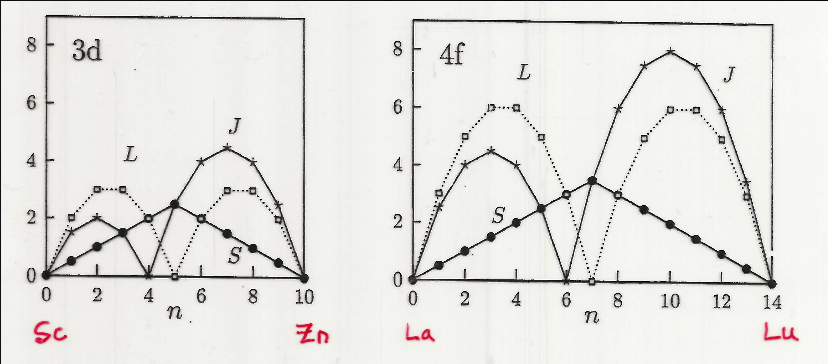
\includegraphics[scale=0.5]{hund.png}
\end{figure}
\begin{equation}
    \chi = \frac{n\mu_0\mu_{eff}^2}{3k_BT}
\end{equation}
means a measure of susceptibility allows us to deduce the effective moment
\begin{equation}
    p = \frac{\mu_{eff}}{\mu_B}
\end{equation}
\begin{figure}[H]
    \centering
    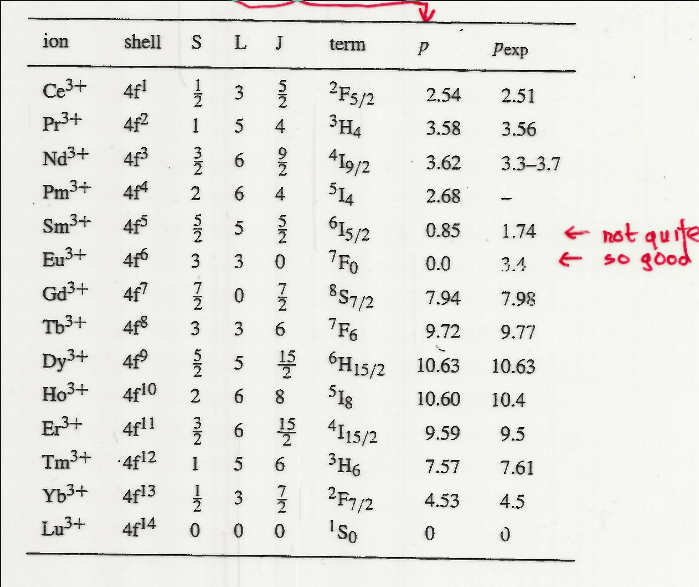
\includegraphics[scale=0.4]{mueff.png}
\end{figure}
Very close agreement between $p$ predicted by Hund's rules and $p_{exp}$.
$Sm^{3+}$ and $Eu^{3+}$ not perfect due to low-lying excited states with higher J.
\begin{figure}[H]
    \centering
    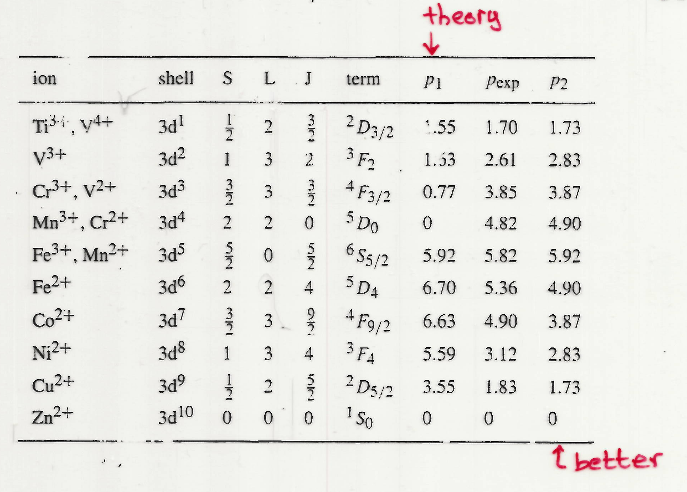
\includegraphics[scale=0.4]{mueff2.png}
\end{figure}
Hund's rules predict 
\begin{equation}
    p = g_J\sqrt{J(J+1)}
\end{equation}
but fit not as good for 3d shell.
This is because of the local crystal environment (crystal field interactions) is much stronger than spin-orbit coupling (Hund's third rule).
Instead the systems choose
\begin{align}
    L = 0 &\to J = S,\, g_J = 2 \\
    \mu_{eff} &= 2\mu_B\sqrt{S(S+1)} \\
    p_2 &= 2\sqrt{S(S+1)}
\end{align}
Orbital quenching. 

\section{Paramagnetic Susceptibility of Conduction Electrons: Pauli Paramagnetism}
Each k-state can be doubly occupied (spin).
Therefore, each electron in a metal is either up or down. 
When a magnetic field is applied to a metal, the energy of the states is either raised or lowered - depending on its spin.
This gives rise to a paramagnetic susceptibility of the electron gas, known as \textbf{Pauli Paramagnetism.}
We might expect that as free electrons are excited into unfilled states to get a Curie-type paramagnetic contribution,
\begin{equation}
    M = \frac{N\mu_B^2B}{k_BT}
\end{equation}
The probability of an electron being line up parallel to B exceeds the probability of anti-parallel orientation by $\approx \frac{\mu_BB}{k_BT}$, thus (8.7).
But Pauli paramagnetism is very small and independent of temperature.
Neglecting the orbital contribution, taking $g=2$, we also ignore the thermal smearing of the Fermi surface at finite temperatures. 
As shown in a magnetic field, the electron band is spin-split into two spin sub-bands separated by $g\mu_BB = 2\mu_BB$.
We willassume that this energy difference is small. 
The number of extra electrons per unit volume with spin up/down is 
\begin{align}
    n_{up} &= \frac12 g(E_F)\mu_BB \\
    n_{down} &= \frac12 g(E_F)\mu_BB
\end{align}
Thus, the magnetisation is given by
\begin{equation}
    M = \mu_B(n_{up} - n_{down}) = g(E_F)\mu_BB
\end{equation}
and the Pauli susceptibility
\begin{align}
    \chi_P = \frac{M}{H} \approx \frac{\mu_0M}{B} = \mu_0\mu_B^2g(E_F) = \frac{3n\mu_0\mu_B^2}{2E_F}
\end{align}
Because the density of states at the Fermi energy is
\begin{equation}
    g(E_F) = \left(\frac{dn}{dE}\right)_{E_F} = \frac32\frac{n}{E_F}
\end{equation}
\begin{figure}[H]
    \centering
    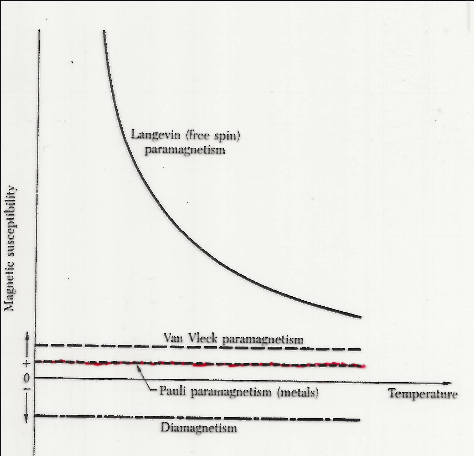
\includegraphics[scale=0.5]{paulmag.png}
\end{figure}
Our prediction for Pauli paramagnetism is temp independent and results in a very small positive susceptibility. 
This is because when we apply a magnetic field to a metal, most of the conduction electrons cannot invert their spin-filled states. 
Only electrons within $k_BT$ of the top of the Fermi-Dirac distribution ($\approx 1\%$) have a chance to invert their spin.
A tiny number which is temperature independent.

\section{Ferromagnetism}
A ferromagnet has a spontaneous magnetic moment - a magnetic moment even in zero applied magnetic field. 
This suggests that the electron spins and magnetic moments are aligned in a regular order.
\begin{figure}[H]
    \centering
    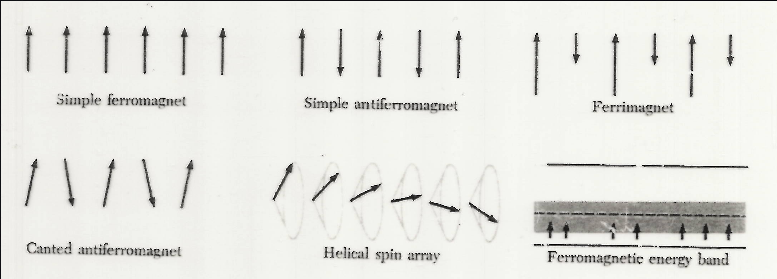
\includegraphics[scale=0.5]{ferro.png}
\end{figure}
There are many different types of magnetic order, and more are being discovered.

\section{Classical Molecular Field Theory}

Weiss postulated that there was an internal magnetic field, or exchange field, $B_E$, within a ferromagnetic material with a flux density proportional to the magnetisation of the material, 
\begin{equation}
    \B_E = \mu_0N_W\unl{M}
\end{equation}
where $N_W$ is the molecular field constant. 
In the mean field approximation, we assume each magnetic atom (or ion) experiences a field proportional to the magnetisation
\begin{equation}
    \B_E = \lambda\unl{M}
\end{equation}
where $\lambda$ is a constant, independent of temperature.

The paramagnetic phase of a ferromagnet occurs at high temperatures well above the Curie temperature, i.e. $T > T_C$.
At this temperature, there is no spontaneous magnetic order, but an applied magnetic field can induce a finite magnetisation, which through the molecular field, acts to further modify the magnetisation.
\begin{equation}
    \mu_0\unl{M} = \chi_p(\B_0 + \mu_0N_W\unl{M}) = \chi_p(\B_0 + \B_E)
\end{equation}
where $\B_0 = \mu_0H$ and $\chi_p$ is the paramagnetic susceptibility. 
We can treat it as if the paramagnet was in a magnetic field, $\B_0 + \B_E$.
At low temperatures, the moments can be aligned by the internal molecular field, even without any applied magnetic field - it is self-sustaining. 
As the temperature is raised, thermal fluctuations begin to progressively destroy the magnetisation.
This is the \textbf{Weiss model of ferromagnetism}.
We solve simultaneously:
\begin{align}
    \frac{M}{M_s} &= B_J(y) & y &= \frac{g_J\mu_BJ(B + \lambda M)}{k_BT}
\end{align}
\begin{figure}[H]
    \centering
    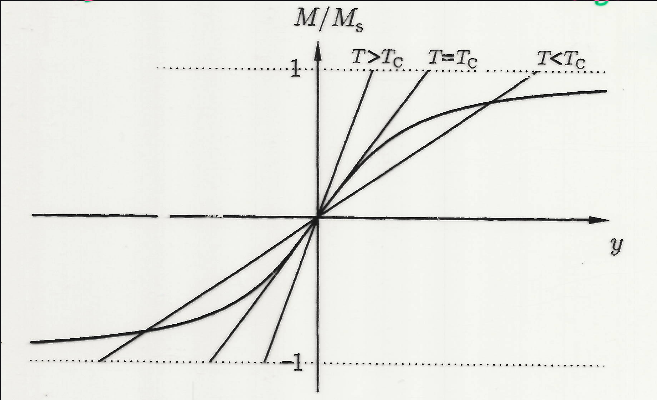
\includegraphics[scale=0.5]{janet.png}
\end{figure}
At $B=0$,
\begin{equation}
    M = \frac{k_BTy}{g_J\mu_BJ\lambda}
\end{equation}
Hence the line of $M$ against $y$ has a gradient which is proportional to temperature. 
The temperature at which the transtion occurs can be found when the gradients of 
\begin{align}
    M &= \frac{k_BTy}{g_J\mu_BJ\lambda M_s} & M &= M)SB_J(y) 
\end{align}
are equal at the origin.
For small $y$,
\begin{equation}
    B_J(y) = \frac{(J+1)y}{3J} + O(y^3)
\end{equation}
The transition temperature, known as the \textbf{Curie temperature} is then
\begin{equation}
    T_C = \frac{g_J\mu_B(J+1)\lambda M_s}{3k_B} = \frac{n\lambda\mu_{eff}}{3k_B}
\end{equation}
The molecular field
\begin{equation}
    \B_E = \lambda M_s = \frac{3k_BT_C}{g_J\mu_B(J+1)}
\end{equation}
so for a ferromagnet like iron, 
\begin{align}
    J &= \frac12,~ T_C \approx 10^3\,K \\
    \B_E &= \frac{k_BT_C}{\mu_B} \approx 1500\,T
\end{align}
This is an enormous effective magnetic field and reflects the size of the Heisenberg exchange interaction.
The exchange field in iron is very much stronger than the real magnetic field due to the other magnetic atoms/ions in the crystal. 
A magnetic atom produces a field $\approx \frac{\mu_B}{a^3}$, or about $0.1$T at a neighbouring atom.

\chapter{}
\section{The Exchange Interaction}
The charge distribution of a system of two spins depends on whether the spins are parallel or antiparallel. 
The Pauli principle excludes two electrons of the same spin from being at the same place at the same time.
It does not exclude two electrons of opposite spin. 
Thus the electrostatic energy of a system will depend on the relative orientation of the spins. 
This \textbf{exchange interaction} is purely electrostatic and is the reason that the molecular field appears so high. 
We can incorporate the exchange interaction into Schrodinger's equation by writing the Hamiltonian of the Heisenberg model to be 
\begin{equation}
    \Ham = -2\sum_{i>j} J_{ij}\unl{S}_i \unl{S}_j
\end{equation}
hence the exchange energy is
\begin{equation}
    U = -2J\unl{S}_i\unl{S}_j
\end{equation}
where $J_{ij}$ or $J$ is the exchange integral and is related to the overlap of the charge distributions of the atoms $i,j$.
We can establish an approximate relationship between the exchange integral $J$ and the Curie temperature, $T_C$.
For an atom having $z$ nearest neighbours and an exchange interaction $J$ then mean field theory gives
\begin{equation}
    J = \frac{3k_BT_C}{2zS(S+1)}
\end{equation}
Using this for iron ($S=1,z=8$), the observed Curie temperature ($T_C = 1043$) gives $J = 11.9\,meV$ - a rather small magnetic exchange interaction. 
\begin{figure}[H]
    \centering
    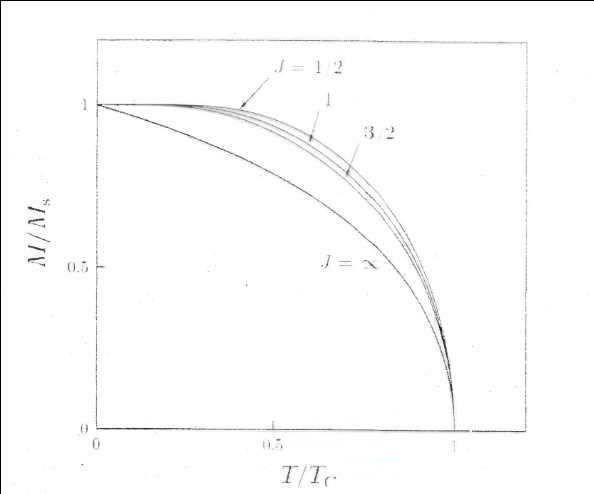
\includegraphics[scale=0.5]{exchange.png}
\end{figure}
We can compare our prediction of how the magnetisation varies as a function of temperature (or reduced temperature $T/T_C$).
The data fits well for Gd ($J=8$) and varies with the angular momentum of the particles. 
\begin{figure}[H]
    \centering
    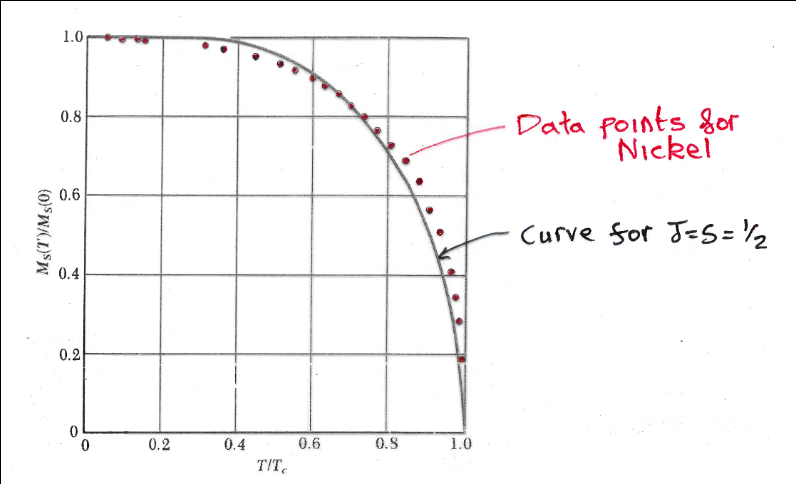
\includegraphics[scale=0.5]{nick.png}
\end{figure}
The data fits quite well for Iron, Cobalt, Nickel, but does not fit at very low temperatures. 
Experimentally, it is found that the best fit is
\begin{equation}
    \frac{\Delta M}{M(0)} = AT^{3/2}
\end{equation}
where $A$ is a sample-dependent constant. 
The reason for this discrepancy is that the Weiss model considers only the ground state.
It does not include low-energy excitations which reduce the magnetisation by forming \textbf{spin waves.}

\section{Spin Waves}
The ground state of a simple ferromagnet has all the spins parallel at $T=0$ as shown below. 
\begin{figure}[H]
    \centering
    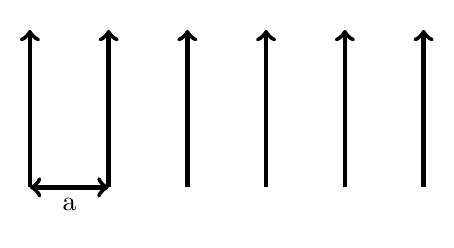
\begin{tikzpicture}
        \draw[ultra thick,->] (-3,0) -- (-3,2);
        \draw[ultra thick,<->] (-3,0) -- (-2,0) node[anchor=north,midway] {a};
        \draw[ultra thick,->] (-2,0) -- (-2,2);
        \draw[ultra thick,->] (-1,0) -- (-1,2);
        \draw[ultra thick,->] (0,0) -- (0,2);
        \draw[ultra thick,->] (1,0) -- (1,2);
        \draw[ultra thick,->] (2,0) -- (2,2);
    \end{tikzpicture}
\end{figure}
Consider a line, or ring, of $N$ ions each with spin $S$ coupled by the Heisenberg interaction
\begin{equation}
    U = -2J\sum_{i=1}^N \unl{S}_i\cdot \unl{S}_{i+1}
\end{equation}
where $J$ is the exchange integral and $\hbar\unl{S}_i$ is the angular momentum of the spin at site $i$.
Treating the spins as classical vectors then $\unl{S}_i\cdot\unl{S}_{i+1} = S^2$ and hence the exchange energy at $T=0$ will be 
\begin{equation}
    U_0 = -2NJS^2
\end{equation}
\begin{figure}[H]
    \centering
    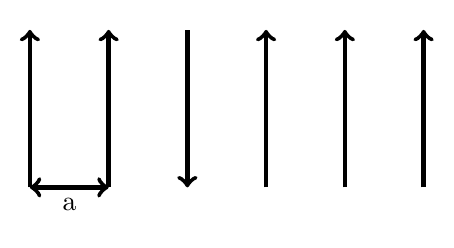
\begin{tikzpicture}
        \draw[ultra thick,->] (-3,0) -- (-3,2);
        \draw[ultra thick,<->] (-3,0) -- (-2,0) node[anchor=north,midway] {a};
        \draw[ultra thick,->] (-2,0) -- (-2,2);
        \draw[ultra thick,<-] (-1,0) -- (-1,2);
        \draw[ultra thick,->] (0,0) -- (0,2);
        \draw[ultra thick,->] (1,0) -- (1,2);
        \draw[ultra thick,->] (2,0) -- (2,2);
    \end{tikzpicture}
\end{figure}
According to the Weiss model, the first excited state of the system will be when a single spin flips. 
However, this rasies the energy of the system to
\begin{equation}
    U = U_0 + 8JS^2
\end{equation}
There is, however, a much lower energy excitation available, one in which the reversal energy is shared between many spins. 
This excitation, \textbf{a spin wave}, has the ends of the spin vectors precessing on the surface of cones, with successive spins advanced in phase by a small constant angle. 
\begin{figure}[H]
    \centering
    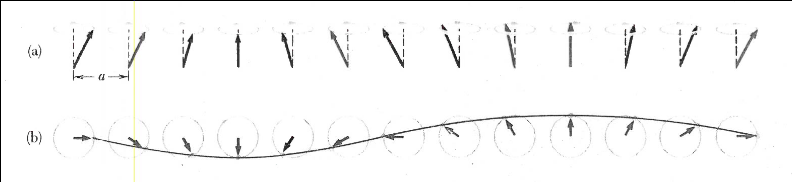
\includegraphics[scale=0.5]{precess.png}
\end{figure}
These spin waves are analagous to lattice vibrations. 
Spin waves are collective oscillations in the relative orientations of spin on a lattice. 
Lattice vibrations are collective oscillations in the relative positions of atoms around lattice sites. 
Spin waves disperse just as lattice vibrations do. 
As in Level 2, we cand erive the spin wave dispersion of an isotropic ferromagnetic. 
\begin{equation}
    \hat{\Ham} = -2J\sum_i \unl{\hat{S}}_i\cdot\unl{\hat{S}}_{i+1}
\end{equation}
The time dependence of the expected value of an operator
\begin{align}
    \frac{d\langle \hat{A}\rangle}{dt} &= \frac{1}{i\hbar}\langle[\hat{A},\hat{\Ham}]\rangle \\
    \frac{d\langle\unl{\hat{S}}\rangle}{dt} &= \frac{1}{i\hbar}\langle[\hat{S},\hat{\Ham}]\rangle = \frac{2J}{\hbar}\langle \unl{\hat{S}}_j\times\left(\unl{\hat{S}}_{j-1} + \unl{\hat{S}}_{j+1}\right)\rangle
\end{align}
Treating the spins at each site as classical vectors. 
The ground state ($T=0$) has all the spins aligned along the $z$-axis:
\begin{align}
    S_j^z &= 0 & S_j^x &= S_j^y = 0
\end{align}
Consider a state which involves a small departure from this
\begin{align}
    S_j^z &\approx S & S_j^x,S_j^y &<< S
\end{align}
then 
\begin{align}
    \frac{dS_j^x}{dt} &\approx \frac{2JS}{\hbar}(2S_j^y - S_{j-1}^y - S_{j+1}^y) \\
    \frac{dS_j^y}{dt} &\approx -\frac{2JS}{\hbar}(2S_j^x - S_{j-1}^x - S_{j+1}^x) \\
    \frac{dS_j^z}{dt} &\approx 0
\end{align}
The solutions to these rate equations have the form of normal mode solutions
\begin{align}
    S_j^x &= Ae^{i(qja-\omega t)} & S_j^y &= Be^{i(qja-\omega t)}
\end{align}
where $q$ is the wavevector. 
By substitution, we can show $A = iB$ such that the $x$ and $y$ motions are $\frac{\pi}{2}$ out of phase and hence
\begin{equation}
    \hbar\omega = 4JS(1-\cos(qa))
\end{equation}
This is the spin wave dispersion curve, reminiscent of the lattice vibration dispersion curve.
\begin{figure}[H]
    \centering
    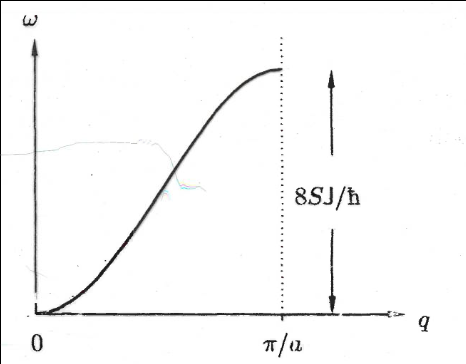
\includegraphics[scale=0.5]{spinwave.png}
\end{figure}

\section{Magnons}
Just as lattice vibrational energy is quantised into packets called \textbf{phonons}, then our spin waves at low temperatures are quantised into \textbf{magnons.}
These magnons are long-wavelength massless excitations and are an example of a Goldstone mode or boson. 
So let us derive the dispersion of magnons using quantum mechanics. 
In one dimension, we can write the Hamiltonian,
\begin{equation}
    \hat{\Ham} = -2J\sum_i\left[\hat{S}_i^z\hat{S}_{i+1}^z + \frac12\left(\hat{S}_i^+\hat{S}_{i+1}^- + \hat{S}_i^-\hat{S}_{i+1}^+\right)\right]
\end{equation}
so that
\begin{equation}
    \hat{\Ham}|\phi\rangle = -NS^2J|\phi\rangle
\end{equation}
Now to create an excitation, we flip a spin at site $j$
\begin{align}
    |\phi\rangle &= \uparrow\uparrow_j\uparrow\uparrow\uparrow\uparrow \\
    |j\rangle &= \uparrow\downarrow\uparrow\uparrow\uparrow\uparrow 
\end{align}
Let us consider $|j\rangle$ which is the ground state of the new system. 
By flipping a spin, we have changed the total spin of the system by $\frac12 - (-\frac12) = 1$.
So this excitation has integer spin and is a boson. 
Applying the Hamiltonian
\begin{equation}
    \hat{\Ham}|j\rangle = 2\left[-NS^2J + 2SJ|j\rangle - SJ|j+1\rangle - SJ|j-1\rangle\right]
\end{equation}
We note that this is not a multiple of $|j\rangle$ so this state is not an eigenstate of the Hamiltonian. 
Nevertheless, we can diagonalise the Hamiltonian by looking for plane-wave solutions of the form
\begin{equation}
    |q\rangle = \frac{1}{\sqrt{N}}\sum_j e^{iqR_j}|j\rangle
\end{equation}
The state $|q\rangle$ is essentially a flipped spin delocalised over all the sites. 
Since it is composed of states representing a single flipped spin, the total spin of $|q\rangle$ is $NS-1$.
Then 
\begin{align} 
    \hat{\Ham}|q\rangle &= E(q)|q\rangle \\
    E(q) = -2NS^2J + 4JS(1-\cos(qa))
\end{align}
The energy of the excitation is then
\begin{equation}
    \hbar\omega = 4JS(1-\cos(qa))
\end{equation}
which is the same result as the classical spin wave dispersion. 
Returning to our dispersion curve, we note that in the long wavelength limit ($qa << 1$), the dispersion relation is
\begin{equation}
    \omega \approx \left(\frac{2JSa^2}{\hbar}\right)q^2
\end{equation}
In the case of a 3D cubic ferromagnet (such as iron), each atom has $z$ nearest neighbours. 
\begin{equation}
    \omega = \left(\frac{2JS}{\hbar}\right)\left[z - \sum_r\cos(\unl{q}\cdot\unl{q})\right]
\end{equation}
where $r$ is a vector joining the central atom to its $z$ neighbours. 
The energy of a spin wave of frequency $\omega$ is 
\begin{equation}
    E(\omega) = (n_q + \frac12)\hbar\omega
\end{equation}
where $n_q$ is the number of magnons. 
The magnons are thermally excited and at thermal equilibrium, their average number is given by the \textbf{Planck distribution.}
\begin{equation}
    \langle n_q\rangle = \frac{1}{\exp\left(\hbar\omega_q/k_BT\right) - 1}
\end{equation}
The total number of magnons excited at a temperature $T$ is 
\begin{equation}
    \sum_q n_q = \int D(\omega)\langle n(\omega)\rangle\,d\omega
\end{equation}
where $D(\omega)$ is the number of magnons per unit frequency range. 
We integrate over the allowed range of $q$ (the first Brillouin zone), and at low temperatures, we may evaluate the integral between $0$ and $\infty$ because $\langle n(\omega)\rangle \to 0$ exponentially as $\omega\to\infty$.

\chapter{}
Magnons have a single polarisation for each $q$.
So using the density of states in 3 dimensions.
\begin{align}
    D(\omega)\,d\omega &= \left(\frac{1}{2\pi}\right)^3 V(4\pi q^2)\,d\omega \\
                       &= \left(\frac{1}{2\pi}\right)^3 \frac{V}{2} \left(4\pi \frac{\hbar\omega}{2JSa^2}\right)\left(\frac{\hbar}{2JSa^2}\right)^{1/2}\frac{1}{\omega^{1/2}}\,d\omega \\
                       &= \left(\frac{1}{4\pi^2}\right)V\left(\frac{\hbar}{2JSa^2}\right)^{3/2}\omega^{1/2}\,d\omega
\end{align}
and hence using (9.30) and (9.31)
\begin{align}
    \sum_q n_q &= \frac{V}{4\pi^2}\left(\frac{\hbar}{2JSa^2}\right)^{3/2} \ofnt \frac{\omega^{1/2}}{\exp\left(\frac{\hbar\omega}{k_BT}\right)-1}\,d\omega \\
               &= \frac{V}{4\pi^2}\left(\frac{k_BT}{2JSa^2}\right)^{3/2} \underbrace{\ofnt \frac{x^{1/2}}{\exp(x) - 1}\,dx}_{0.0587\times4\pi^2},~ x = \frac{\hbar\omega}{k_BT}
\end{align}
Noting that the spin angular momentum can only change by one quantum unit for each spin wave created then the magnetic moment change.
\begin{equation}
    g\mu_B\sum_qn_q = g\mu_BV\left(\frac{k_BT}{2JSa^2}\right)^{3/2}\times0.0587
\end{equation}
and hence the magnetisation will be
\begin{align}
    \Delta M = M_{sat} - M(T) &= \frac{g\mu_B\sum_qn_q}{V} \\
                              &= g\mu_B\left(\frac{k_BT}{2JSa^2}\right)^{3/2}\times0.0587
\end{align}
and the fractional change will be
\begin{equation}
    \frac{\Delta M}{M_{sat}} = \frac{g\mu_B\left(\frac{k_BT}{2JSa^2}\right)^{3/2}\times0.0587}{ng\mu_BS} = \frac{1}{nS}\left(\frac{k_BT}{2JSa^2}\right)^{3/2}\times0.0587 
\end{equation}
where $n$ is the number of atoms per unit volume, $n=\frac{N}{V}$.
\begin{example}[Nickel]
    Nickel has a fcc structure - 4 atoms per unit cell. 
    \begin{align}
        n &= \frac{4}{a^3} \\
        \frac{\Delta M}{M_{sat}} &= \frac{1}{4S}\left(\frac{k_BT}{2JS}\right)^{3/2}\times0.0587 
    \end{align}
    Taking $S=1$ ($L=0$, quenched orbital angular momentum) and $\Delta M/M_{sat} \approx 5\times10^{-3}$ at $60\,K$ gives
    \begin{equation}
        J = \left(\frac{0.0587}{4S(\Delta M/M_{sat})}\right)^{3/2} \left(\frac{k_BT}{2S}\right) = 8.5\times10^{-22}\;\text{Joules}
    \end{equation}
\end{example}
Note that (10.9) is Bloch's experimentally observed $T^{3/2}$ law. 
The energy of the magnon modes is given by 
\begin{equation}
    E_{magnon} = \ofnt \frac{\hbar\omega\,g(\omega)\,d\omega}{\exp\left(\frac{\hbar\omega}{k_BT}\right) - 1} \propto T^{5/2}
\end{equation}
So that the heat capacity,
\begin{equation}
    C = \frac{\p E_{magnon}}{\p U} \propto T^{3/2}
\end{equation}
\begin{figure}[H]
    \centering
    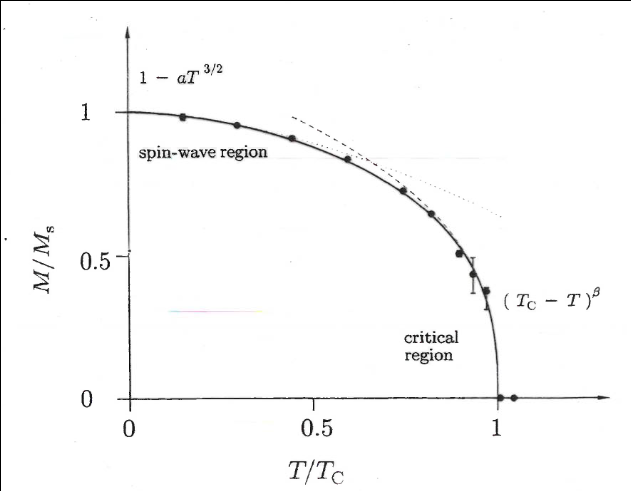
\includegraphics[scale=0.5]{critspin.png}
\end{figure}

\section{Magnetic Domains}
Even in ferromagnets with a large exchange integral $J$, we find a number of magnetic domains. 
Within each domain, the local magnetisation reaches $M_{sat}$ but overal the sample may have $M\approx 0$.
Domains are separated by domain walls.
Domain walls need not be parallel, or even straight.
\begin{figure}[H]
    \centering
    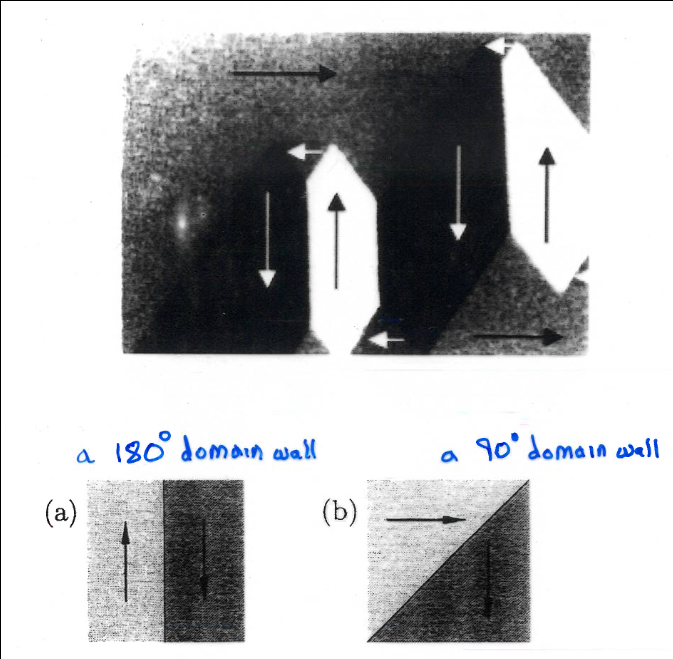
\includegraphics[scale=0.4]{domain.png}
\end{figure}
The existence of domains, and domain walls, can explain why some ferromagnets may have $M\approx 0$ even though they are spontaneously magnetised and increase saturation magnetisation by applying a tiny ($10^{-6}$T) applied field - \textbf{domain wall motion.}
The most common type of $180^\circ$ domain wall is a \textbf{Bloch wall.}
\begin{figure}[H]
    \centering
    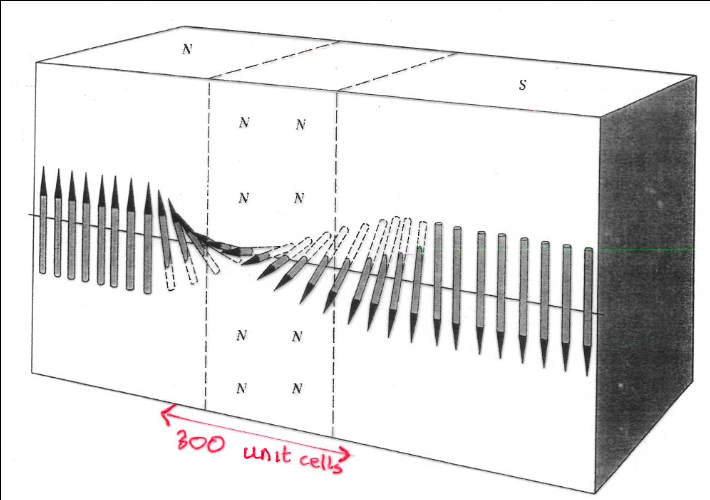
\includegraphics[scale=0.5]{blochwall.png}
\end{figure}
It is not atomically sharp. 
The magnetisation rotates in a plane parallel to the plane of the wall. 
In iron, the 'thickness' of the wall is about 300 unit cells.
\begin{figure}[H]
    \centering
    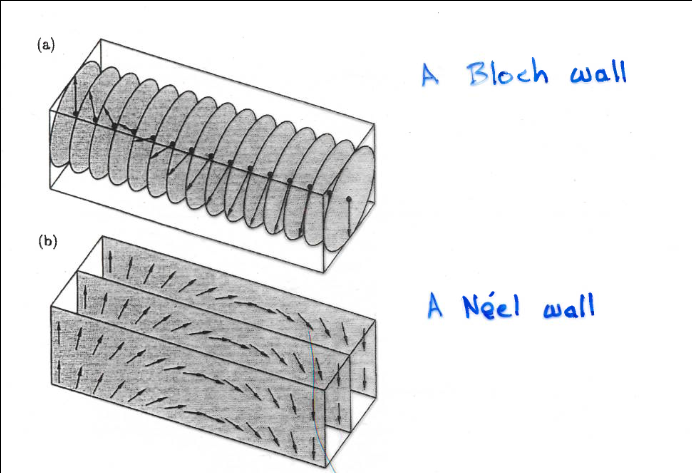
\includegraphics[scale=0.5]{walls.png}
\end{figure}
Let us try and calculate the thickness of a Bloch wall. 
In a ferromagnet, it costs energy to rotate neighbouring spins. 
Two spins, $\unl{S}_1$ and $\unl{S}_2$, which are at an angle of $\theta$ to each other, have an energy $-2J\unl{S}_1\cdot\unl{S}_2 = -2JS^2\cos\theta$. 
If $\theta=0$, their energy is $-2JS^2$.
As $\cos\theta \approx 1-\frac{theta^2}{2}$ for $\theta << 1$, then the energy cost for $\theta\neq0$ is $JS^2\theta^2$ if $\theta<<1$.
In a Bloch wall, spins rotate over $N$ sites by an angle $\pi$. 
Hence the energy cost of a line of spins is equal to $N$ contributions of $JS^2\theta^2$, where $\theta=\frac{\pi}{N}$, i.e. to $J^2S^2\frac{\pi^2}{N}$.
In a Bloch wall, we have planes of spins and so we are interested in $\sigma_{BW}$, the energy per unit area of the Bloch wall. 
In a square metre of wall, there are $\frac{1}{a^2}$ lines of spins. 
Hence,
\begin{equation}
    \sigma_{BW} = JS^2\frac{\pi^2}{Na^2}
\end{equation}
Which means a Bloch wall would be unstable - it would unwind itself growing in size throughout the entire sample. 
This is because it costs energy to twist spins - what is stopping them from unwinding?

\section{MAgnetocrystalline Anisotropy}
Crystals possess a magnetic \textbf{'easy axis'} and a \textbf{'hard axis'.}
\begin{figure}[H]
    \centering
    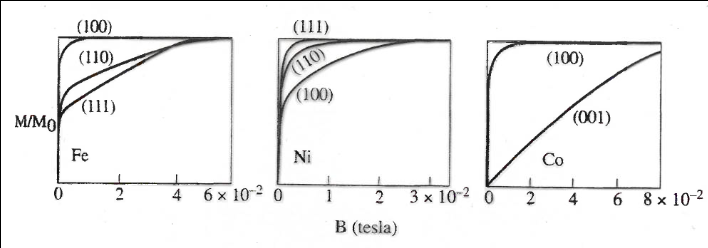
\includegraphics[scale=0.5]{axes.png}
\end{figure}
Along certain crystallographic directions, it is easy to magnetise sample, along others it is more difficult (requiring higher fields).
This is due to a potential energy which depends upon the direction of magnetisation - \textbf{the magnetocrystalline anisotropy energy, $E_{anis}$.}
For cubic systems, 
\begin{equation}
    U_{anis} = K_1(\alpha_1^2\alpha_2^2 + \alpha_1^2\alpha_3^2 + \alpha_2^2\alpha_3^2) + K_2(\alpha_1^2\alpha_2^2\alpha_3^2)
\end{equation}
where $\alpha_1 = \cos\theta_1$, $\alpha_2=\cos\theta_2$, $\alpha_3=\cos\theta_3$ are the direction cosines of the magnetisation direction with respect to the edges of the cubic unit cell, and $K_1$ and $K_2$ are the anisotropy constants.
When $K_1>0$ (e.g. iron), the easy axis is along $\langle 100\rangle$ and other directions, $\langle 111\rangle$ are hard.
When $K_1<0$ (e.g. nickel), the easy axis is $\langle111\rangle$ and $\langle100\rangle$ is hard.\\
Magnetocrystalline anisotropy is a consequence of a combination of spin-orbit coupling and the interaction of the orbits with the crystal field.
\begin{figure}[H]
    \centering
    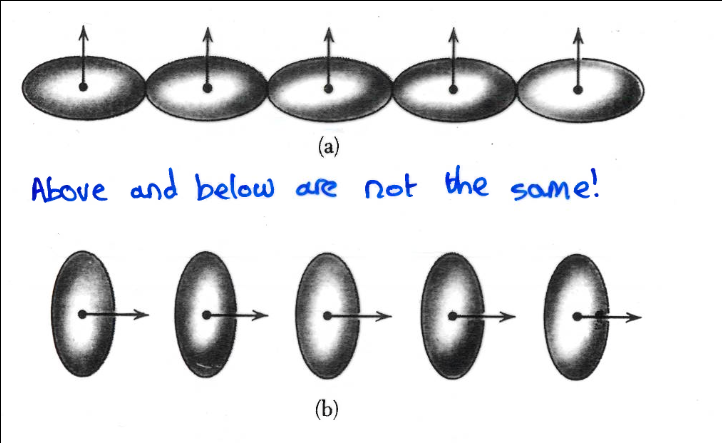
\includegraphics[scale=0.5]{anis.png}
\end{figure}

\section{Domain Wall Width (Again)}
In the magnetic domains, the magnetisation will prefer to lie along the easy axis. 
But in the domain wall, it will have to rotate, and a component will lie along the hard axis - costing energy. 
We assume a simple form for the anisotropy energy density
\begin{equation}
    E_{anis} = K\sin^2\theta
\end{equation}
where $K$ is an anisotropy constant.
We take $K>0$ so that the spins align up along $\theta=0,\pi$.\\
We add up the contribution from each of the $N$ spins as an integral.
The energy density contribution to the Bloch wall is 
\begin{equation}
    \sum_{i=1}^N K\sin^2\theta_i = \frac{N}{\pi} \int_0^\pi K\sin^2\theta\,d\theta = \frac{NK}{2}
\end{equation}
The energy contribution per unit area is then $\frac{NKa}{2}$.
Thus the total energy including the exchange energy and the anisotropy energy is
\begin{equation}
    \sigma_{BW} = JS^2\frac{\pi^2}{Na^2} + \frac{NKa}{2}
\end{equation}
This is much better!
The first term $\propto \frac{1}{N}$ tends to unwind the wall and make it bigger, but the second term $\propto N$ tends to tighten it and make it smaller. 
The equilibrium configuratino using $\frac{dE}{dN} = 0$ gives
\begin{equation}
    N = \pi S\sqrt{\frac{2J}{Ka^3}}
\end{equation}
Typically for iron, $N=300$. 
The width of the Bloch wall is then
\begin{equation}
    \delta = Na = \pi S\sqrt{\frac{2J}{Ka}}
\end{equation}
where $a$ is the lattice parameter. 
Note that a larger $J$ makes the domain wall thicker whilst a larger anisotropy $K$ makes it smaller. 
The energy per unit area of the domain wall is 
\begin{equation}
    \sigma_{BW} = \pi S\sqrt{\frac{2JK}{a}}
\end{equation}

\chapter{}
\section{Domain Formation}
Making a domain wall costs energy. 
So why do we have more than one domain?
The reason is that the formation of domains saves energy associated with dipolar fields. 
Because $\del\cdot\unl{H} = -\del\cdot\unl{M}$ then whenever $\unl{M}$ stops and starts (e.g. at the edges of a sample), the magnetic field diverges, producing demagnetising fields filling space and costing $\frac{B^2}{2\mu_0}$ Joules of energy per $m^2$.
The energy associated with the demagnetising field is called the \textbf{demagnetisation energy:}
\begin{equation}
    -\frac{\mu_0}{2}\int_V \unl{M}\cdot\unl{H}_d\,d\tau 
\end{equation}
where $\unl{H}_d$ is the demagnetising field and the integral is taken over the volume of the sample. 
For an ellipsoidally-shapped sample magnetised along a principle axis, this energy reduces to
\begin{equation}
    \frac{\mu_0}{2}NM^2V
\end{equation}
where $N$ is the demagnetising factor and $V$ is the sample volume. 
This demagnetisation energy can be saved by breaking into domains - but each domain created costs energy because of the domain walls. 
\begin{figure}[H]
    \centering
    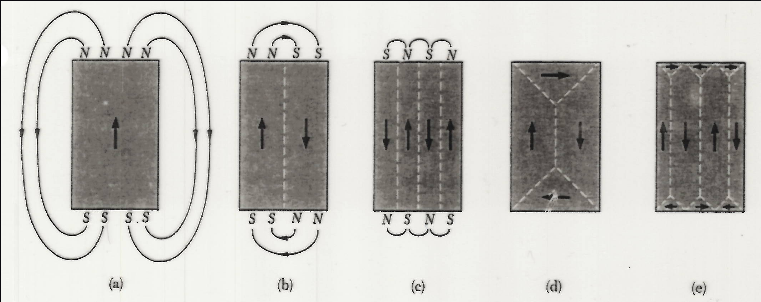
\includegraphics[scale=0.5]{demag.png}
\end{figure}
In (a), the sample has no domain walls but a large demagnetisation energy. 
This can be reduced by forming 2 domains (b) or 4 domains (c) - at a cost of making domain walls. 
Closure of domain walls in (d) and (e) eliminate demagnetisation energy but form further domain walls. 
Note that within a domain, the magnetisation will be along the easy axis.

\section{Magnetisation Processes}
The figure shows a typical hysteresis loop found when measuring the magnetisation as a function of the applied magnetic field for a ferromagnet.
\begin{figure}[H]
    \centering
    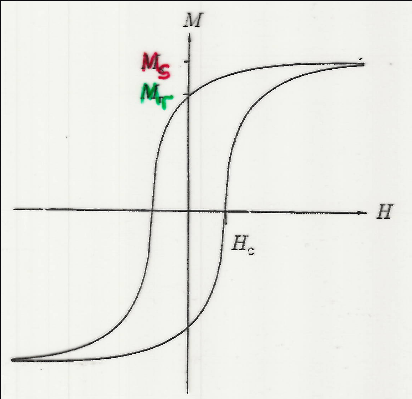
\includegraphics[scale=0.5]{process.png}
\end{figure}
\begin{wrapfigure}{r}{0.4\textwidth}
    \centering
    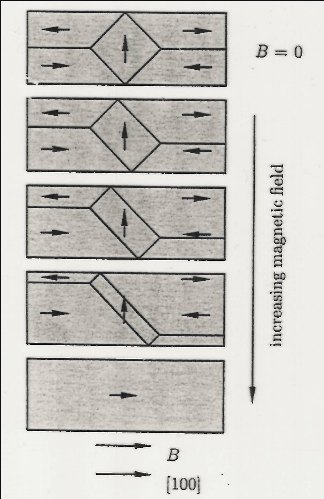
\includegraphics[scale=0.4]{incmag.png}
\end{wrapfigure}
If the sample is magnetised to $M_S$ by an applied field then when the applied field is reduced to zero, the magnetisation is reduced to the remnant magnetisation, $M_r$.
A magnetic field equal to the coercive field $H_c$ is needed to switch the magnetisation. 
When a demagnetised ferromagnet is magnetised, various process occur: \\
First is domain wall motion. 
Domains aligned to the applied field will grow in size at the expense of domains unfavourably aligned.\\
Second, at higher fields, domain rotation can occur, overcoming the anisotropy energy. \\
Finally, at the highest magnetic fields is coherent rotation of the domains to be aligned with the field, overcoming easy and hard axes.

\section{Soft and Hard Magnetic Materials}
The energy (heat) dissipated by a ferromagnet as it is taken around a circuit of the hysteresis loop is proportional to the area enclosed by the loop. 
If the area is small, domain wall motion is easy and the material is \textbf{magnetically soft.}
If the area is large, domain wall motion is very hard and the material is \textbf{magnetically hard.}
The coercivity of a sample is the magnetic field $H_c$ required to reduce the magnetisation to zero.
Coercivities vary greatly:
\begin{center}
    \begin{tabular}{c|l|c|l}
                           & Material & Coercivity & Uses \\
        \hline
        {\color{red} Soft} & Fe-Ni supermalloy & $2\times10^{-7}$T & pulse transformer \\
                           & Si4\%-Fe & $5\times10^{-5}$T & power transformer \\
                           & Alnico V & $0.06$T & loudspeaker magnet \\
        {\color{red} Hard} & SmCo$_5$ & $1.0$T & high field magnet 
    \end{tabular}
\end{center}

\subsection{Soft Magnetic Materials}
Soft magnetic materials are easy to magnetise. 
They have:
\begin{itemize}
    \item a high permeability 
    \item a low $H_c$
    \item small hysteresis loss 
    \item a small $M_r$ 
    \item a high saturation magnetisation
\end{itemize}
Soft magnetic materials have a low coercivity. 
They are used in transformer cores, generators and motors, electromagnets and magnetic 'write' heads.

\subsection{Hard Magnetic Materials}
Hard magnetic materials are difficult to magnetise, and hence difficult to demagnetise. 
Hard magnets are used as permanent magnets (in loudspeakers, in motors, fridge magnets) and in magnetic tape recording.
The energy dissipated in a hysteresis loop cycle is large and hence magnetisation will not occur spontaneously. 
They have:
\begin{itemize}
    \item a low permeability
    \item a high $H_c$
    \item large hysteresis loop
    \item a large $M_r$
    \item a high saturation magnetisation
\end{itemize}

\section{Antiferromagnetism}
There are many different ways of ordering magnetic moments. 
If the exchange interaction is negative, $J<0$, the molecular field is oriented for nearest neighbours to lie \textbf{anti-parallel} to one another. 
We can consider antiferromagnets to be composed of two interpenetrating sublattices.
\begin{figure}[H]
    \centering
    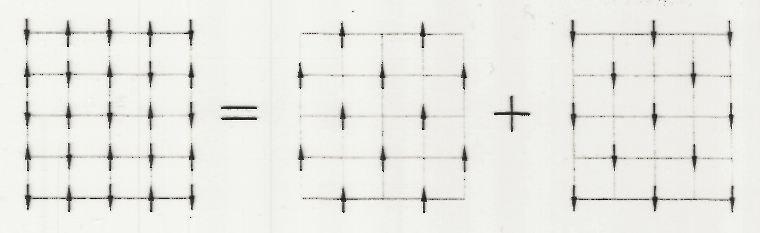
\includegraphics[scale=0.5]{sublat.png}
\end{figure}
Each spin has nearest neighbours composed entirely of the other sublattice.
Initially we will assume the molecular field on one sublattice is proportional to the magnetisation of the other sublattice. 
We will also assume no applied magnetic field. 

\subsection{Weiss Model of an Antiferromagnet}
If we label the 'up' sublattice $+$ and the 'down' sublattice $-$, then the molecular field on each sublattice is
\begin{align}
    B_+ &= -|\lambda|M_- \\
    B_- &= -|\lambda|M_+ 
\end{align}
where $\lambda$ is the molecular field constant, which is now negative.
On each sublattice, the molecular field is
\begin{equation}
    M_\pm = M_sB_J\left(\frac{-g_J\mu_B J|\lambda|M_\mp}{k_BT}\right)
\end{equation}
The two sublattices are equivalent in everything except the direction of the moments.
\begin{equation}
    |M_+| = |M_-| \equiv M
\end{equation}
and hence 
\begin{equation}
    M = M_sB_J \left(-\frac{g_J\mu_B J|\lambda|M}{k_BT}\right)
\end{equation}
which is almost identical to the corresponding equation for ferromagnetism.
Thus we expect the molecular field to follw the same behaviour on both sublattices.
Following (11.7), we find that the molecular field will disappear for temperatures above a transition temperature, \textbf{the Neel temperature,} $T_N$, defined by
\begin{align}
    T_N = \frac{g_J\mu_B(J+1)|\lambda|M_s}{3k_B} = \frac{n|\lambda|\mu^2_{eff}}{3k_B}
\end{align}
Note that although the magnetisation on each sublattice follows the above, the two magnetisations will be in opposite directions so that the net magnetisation, at any temperature, is always zero.

\chapter{}
\section{Magnetic Susceptibility}
For temperatures above $T_N$, the ffect of a small applied magnetic field can be calculated in the same way as for a ferromagnet - (8.20) - by expanding the Brillouin function
\begin{equation}
    B_J(y) = \frac{(J+1)_y}{3J} + O(y^3)
\end{equation}
and results in the magnetic susceptibility being given by 
\begin{equation}
    \chi = \lim_{B\to0} \frac{\mu_0M}{B} \propto \frac{1}{T+T_N}
\end{equation}
which is the Curie-Weiss law, but with the Curie temperature replaced by the Neel temperature. \\
This gives us a means of interpreting susceptibility data in the paramagnetic (high T) state
\begin{equation}
    \chi \propto \frac{1}{T-\theta}
\end{equation}
where $\theta$ is the Weiss temperature. 
If:
\begin{itemize}
    \item $\theta = 0$, then the material is a paramagnet
    \item $\theta > 0$, then the material is a ferromagnet and $\theta = T_C$
    \item $\theta < 0$, then the material is an antiferromagnet and $\theta = -T_N$
\end{itemize}
The Curie-Weiss law states that $\chi \propto \frac{1}{T_\theta}$ for $T>0$.
This is shown for the three cases described above. 
\begin{center}
    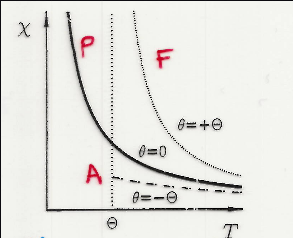
\includegraphics[scale=0.5]{curweiss.png}
\end{center}
Straight-line graphs are obtained by plotting $\frac{1}{\chi}$ against $T$ with the intercept on the y-axis yielding $\theta$.
\begin{center}
    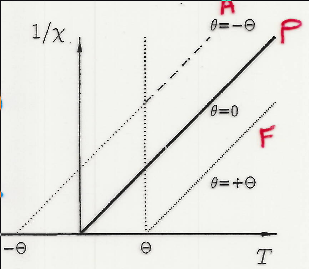
\includegraphics[scale=0.5]{straightcw.png}
\end{center}
A graph of $\chi T$ against $T$ can be constant ($\theta=0$), increasing for decreasing $T$ ($\theta > 0$), or decreasing for decreasing $T$ ($\theta <0$).
\begin{center}
    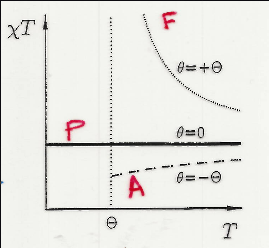
\includegraphics[scale=0.5]{chaitea.png}
\end{center}
Applying a magnetic field to an antiferromagnet at temperatures below $T_N$ is more complicated than the case of a ferromagnet below $T_C$ because the direction is crucial. 
There is no longer any energetic advantage for the moments to align along the field direction because an energy gain on one sublattice is cancelled out by the energy cost for the other sublattice. 

Consider the case at very low $T \sim 0$, where we can ignore thermal fluctuations ($|M_+|$ and $|M_-|$ are both $M_s$).
Applying a small magnetic field parallel to one of the magnetisation will add or subtract a small term to the local field of each sublattice. 
But these are already saturated and thus the net magnetisation, $\chi_{||} = 0$.
If instead, the small magnetic field is applied perpendicular to the magnetisation direction of one of the sublattices, this causes the magnetisation of both sublattices to tilt slightly so that a component of magnetisation is produced along the applied magnetic field direction and hence $\chi_{\perp} \neq 0$.\\
Now consider raising the temperature. 
This causes the molecular field at each sublattice to weaken. 
Thermal fluctuations will greatly affect the magnetic susceptibility when the applied magnetic field is parallel to one of the sublattices, causing the magnetisation of one sublattice to up and the other to down. 
Thus $\chi_{||}$ rises rapidly. \\
However, for perpendicular, there is no effect as $|M_+|$ and $|M_-|$ are affected equally. 
So $\chi_{\perp}$ is independent of temperature.
\begin{center}
    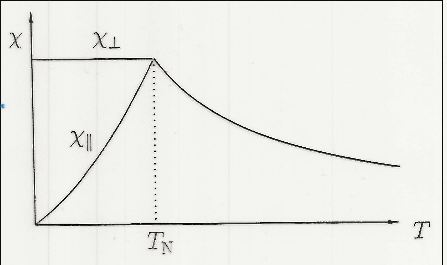
\includegraphics[scale=0.5]{chipar.png}
\end{center}

\section{Ferrimagnetism}
In an antiferromagnet, the net magnetisation at any temperature is zero, as the two sublattices are equivalent and in opposite directions. 
But what if they were not equivalent?
Then we would still have an antiferromagnetic arrangement of spins, but a net mangetic moment - \textbf{Ferrimagnetism.}
Ferrites have formula $MO.Fe_2O_3$, where $M$ is a divalent cation (Zinc, Cobalt, Iron, Nickel, Copper, Manganese, with charge $2+$).
They have a complex crystal structure with 2 types of lattice sites: tetrahedral or octahedral. 

\section{Magnetic Interactions}
\subsection{Magnetic Dipolar Interaction}
Two dipoles $\mu_1$ and $\mu_2$ separated by $\unl{r}$
\begin{equation}
    E = \frac{\mu_0}{4\pi\unl{r}^3}\left[\mu_1\cdot\mu_2 - \frac{3}{r^2}(\mu_1\cdot\unl{r})(\mu_2\cdot\unl{r})\right]
\end{equation}
but very weak, $\mu\approx1\mu_B,\; r\approx0.1nm$.

\subsection{Direct exchange}
If electrons on neighbouring magnetic ions interact via an exchange interaction - \textbf{Direct exchange}.
Also very rare and very weak.
For example, rare earths which have $4f$ electrons are bureid, little probability beyond $0.1\unl{r}$.
For $3d$ transition metals such as Iron, Cobalt, Nickel are metals with conduction electrons, localised and band character need to be considered. 

\subsection{Indirect exchange in ionic solids: Superexchange}
Many ionic solids are magnetic. 
Exchange interaction is too short-ranged, need an indirect exchange over longer distances - superexchange. 
Indirect exchange via oxygen ions.
Superexchange works by lowering energy of electrons by becoming delocalised over the structure, thus lowering kinetic energy.

\subsection{Indirect exchange in metals: Itinerant exchange}
In metals, the exchange interaction between magnetic ions can be mediated by conduction electrons. 
A localised magnetic moment spin polarises the conduction electrons and this polarisation in turn couples to a localised magnetic moment $r$ away. 
\begin{equation}
    J_{Rkky}(r) \propto \frac{\cos(2k_Fr)}{r^3}
\end{equation}
at large $r$.
This interaction is long range and oscillatory. 
Hence depending on the separation, it may be either ferromagnetic or antiferromagnetic.









%\part{}
%%Mendis
%\chapter{}
%\begin{itemize}
%    \item How is a semiconductor different from a metal?
%        \begin{itemize}
%            \item Band Gaps
%        \end{itemize}
%    \item Consider Free Electron Solid 
%        \begin{itemize}
%            \item Zero potential
%                \begin{equation}
%                    E = \frac{\hbar^2k^2}{2m}
%                \end{equation}
%            \item Wavefunction is a plane wave
%                \begin{equation}
%                    \psi(r) = e^{ik\cdot r}
%                \end{equation}
%            \item Energy gap at Brillouin zone boundaries
%            \item Forbidden band due to Bragg reflection at Brillouin zone boundary
%        \end{itemize}
%    \item This won't be a heavy note lecture series
%    \item For some semiconductor alloy of A and B
%        \begin{align}
%            E_{g,AB} &= xE_{g,A} + (1-x)E_{g,B} - bx(1-x) \\
%            a_{AB} &= xa_A + (1-x)a_B 
%        \end{align}
%    \item $b$ is the Bowing parameter
%    \item Equation (1.4) is Vegard's Law
%    \item Key Results
%        \begin{align}
%            F &= \hbar\frac{dk}{dt}, ~v = \frac{1}{\hbar}\frac{dE}{dk} \\
%            m^* &= \frac{\hbar^2}{\frac{d^2E}{dk^2}} \\
%        \end{align}
%    \item For anisotropic crystals (effective mass tensor):
%        \begin{align}
%            m_{ij}^* &= \frac{\hbar^2}{\frac{d^E}{dk_idk_j}}
%        \end{align}
%\end{itemize}
%
%\chapter{}
%Meh, who cares
%
%\chapter{Statistical Mechanics of Semiconductors}
%\begin{itemize}
%    \item N (electrons) is number of energy levels between E and E+dE times the occupation probability for conduction band
%        \begin{align}
%            N &= D(E)\,dE \times f(E) \\
%        \end{align}
%    \item For gap in valence band, i.e. holes
%        \begin{align}
%            N &= D(E)\,dE [1 - f(E)]
%        \end{align}
%    \item Something else, he's actually writing something
%        \begin{align}
%            N &= \int_{E_C}^{E_{max}} D(E)f(E)\,dE \\
%              &= \frac{1}{2\pi^2}\left(\frac{2m}{\hbar^2}\right)^{3/2} \int_{E_C}^\infty \sqrt{E-E_C}\left[\frac{1}{1+\exp\left(\frac{E-\mu}{kT}\right)}\right]\,dE \\
%            \frac{E-\mu}{kT} >> 0 &\implies \frac{1}{1+\exp\left(\frac{E-\mu}{kT}\right)} \approx \exp\left[-\frac{E-\mu}{kT}\right] \\
%            N &= A \int_{E_C}^\infty \sqrt{E-E_C}\exp\left[-\frac{E-\mu}{kT}\right]\,dE \\
%            \exp\left[-\frac{E-\mu}{kT}\right] &= \exp\left[-\frac{E-E_C}{kT}\right]\times\exp\left[\frac{\mu-E_C}{kT}\right] \\
%            N &= A\exp\left[\frac{\mu-E_C}{kT}\right] \int_{E_C}^\infty \sqrt{E-E_C}\exp\left[-\frac{E-E_C}{kT}\right]\,dE \\
%            \mu &= \frac{E-E_C}{kT},~ d\mu = \frac{dE}{kT} \\
%            N &= A\exp\left[\frac{\mu-E_C}{kT}\right](kT)^{3/2} \int_{E_C}^\infty \mu^{1/2}\exp(-\mu)\,d\mu \\
%              &= \left(A(kT)^{3/2}\frac{\sqrt{\pi}}{2}\right)\exp\left[\frac{\mu-E_C}{kT}\right] \\
%            n &= N_C\exp\left[\frac{\mu-E_C}{kT}\right] \\
%              &= N_C\exp\left[-\frac{E_C-\mu}{kT}\right], N_C = 2\left(\frac{m^*_ekT}{2\pi\hbar^2}\right)^{3/2}
%        \end{align}
%    \item Can do the same thing for holes in valence band
%        \begin{equation}
%            p = N_V\exp\left[-\frac{\mu-E_V}{kT}\right], N_V = 2\left(\frac{m^*_hkT}{2\pi\hbar^2}\right)^{3/2}
%        \end{equation}
%    \item $n=p$ in intrinsic semiconductor (no impurities)
%        \begin{equation}
%            \mu = E_{mid-gap} + \frac34 kT\ln\left(\frac{m^*_h}{m^*_e}\right)
%        \end{equation}
%\end{itemize}
%
%\chapter{Extrinsic semiconductor}
%\begin{itemize}
%    \item Doping with foreign atoms to manipulate conductivity
%    \item Donors and acceptors
%    \item Donors give extra electrons, acceptors give extra holes
%    \item Energy level and orbit radius of donor electron
%        \begin{align}
%            E_D &= \frac{e^4m_e^*}{2(4\pi\e_r\e_0\hbar)^2} = \frac{m_e^*}{m\e_r^2}\underbrace{\left[\frac{e^4m}{2(4\pi\e_0\hbar)^2}\right]}_{13.6\,eV} \\
%            r &= \frac{4\pi\e_r\e_0\hbar^2}{m_e^*e^2} = \frac{\e_rm}{m_e^*}\underbrace{\left(\frac{4\pi\e_0\hbar^2}{me^2}\right)}_{\SI{0.5}{\angstrom}}
%        \end{align}
%        \begin{figure}[H]
%            \centering
%            \begin{tikzpicture}
%                \draw[thick,->] (-1.5,0) -- (1.5,0) node[anchor=north west] {k};
%                \draw[thick,->] (0,-3) node[anchor=north] {T = 0} -- (0,3) node[anchor=south east] {E};
%                \draw[thick] (0,-0.5) parabola (-1.5,-3);
%                \draw[thick] (0,-0.5) parabola (1.5,-3);
%                \draw[thick] (0,0.5) parabola (1.5,2.5);
%                \draw[thick] (0,0.5) parabola (-1.5,2.5);
%                \draw[thick] (0,1.5) parabola (1.5,3);
%                \draw[thick] (0,1.5) parabola (-1.5,3);
%                \filldraw (-1.2,-2.2) circle (2pt);
%                \filldraw (-0.9,-1.5) circle (2pt);
%                \filldraw (-0.5,-0.8) circle (2pt);
%                \filldraw (0,-0.5) circle (2pt);
%                \filldraw (1.2,-2.2) circle (2pt);
%                \filldraw (0.9,-1.5) circle (2pt);
%                \filldraw (0.5,-0.8) circle (2pt);
%                \filldraw (-1.2,1.8) circle (2pt);
%                \filldraw (-0.9,1.2) circle (2pt);
%                \filldraw (-0.5,0.7) circle (2pt);
%                \filldraw (0.5,0.7) circle (2pt);
%                \filldraw (0.9,1.2) circle (2pt);
%                \filldraw (1.2,1.8) circle (2pt);
%            \end{tikzpicture}
%            \begin{tikzpicture}
%                \draw[thick,->] (-2,0) -- (2,0) node[anchor=north west] {k};
%                \draw[thick,->] (0,-3) node[anchor=north] {Low T (freeze-out)} -- (0,3) node[anchor=south east] {E};
%                \draw[thick] (0,-0.5) parabola (-2,-3);
%                \draw[thick] (0,-0.5) parabola (2,-3);
%                \draw[thick] (0,0.5) parabola (2,2.5);
%                \draw[thick] (0,0.5) parabola (-2,2.5);
%                \draw[thick] (0,1.5) parabola (2,3);
%                \draw[thick] (0,1.5) parabola (-2,3);
%                \filldraw (-1.7,-2.2) circle (2pt);
%                \filldraw (-1.3,-1.5) circle (2pt);
%                \filldraw (-0.7,-0.8) circle (2pt);
%                \filldraw (0,-0.5) circle (2pt);
%                \filldraw (1.7,-2.2) circle (2pt);
%                \filldraw (1.3,-1.5) circle (2pt);
%                \filldraw (0.7,-0.8) circle (2pt);
%                \filldraw (-1.6,1.8) circle (2pt);
%                \filldraw (-1.2,1.2) circle (2pt);
%                \filldraw[white] (-0.6,0.7) circle (2pt);
%                \draw (-0.6,0.7) circle (2pt);
%                \filldraw (0.6,0.7) circle (2pt);
%                \filldraw[white] (1.2,1.2) circle (2pt);
%                \draw (1.2,1.2) circle (2pt);
%                \filldraw (1.6,1.8) circle (2pt);
%                \draw[->] (-0.6,0.8) -- (-0.6,1.5);
%                \filldraw (-0.6,1.65) circle (2pt);
%                \filldraw (1.2,2.05) circle (2pt);
%                \draw[->] (1.2,1.3) -- (1.2,1.9);
%            \end{tikzpicture}
%            \begin{tikzpicture}
%                \draw[thick,->] (-2,0) -- (2,0) node[anchor=north west] {k};
%                \draw[thick,->] (0,-3) node[anchor=north] {Room T (saturation)} -- (0,3) node[anchor=south east] {E};
%                \draw[thick] (0,-0.5) parabola (-2,-3);
%                \draw[thick] (0,-0.5) parabola (2,-3);
%                \draw[thick] (0,0.5) parabola (2,2.5);
%                \draw[thick] (0,0.5) parabola (-2,2.5);
%                \draw[thick] (0,1.5) parabola (2,3);
%                \draw[thick] (0,1.5) parabola (-2,3);
%                \filldraw (-1.7,-2.2) circle (2pt);
%                \filldraw (-1.3,-1.5) circle (2pt);
%                \filldraw (-0.7,-0.8) circle (2pt);
%                \filldraw (0,-0.5) circle (2pt);
%                \filldraw (1.7,-2.2) circle (2pt);
%                \filldraw (1.3,-1.5) circle (2pt);
%                \filldraw (0.7,-0.8) circle (2pt);
%                \filldraw[white] (-1.6,1.8) circle (2pt);
%                \draw (-1.6,1.8) circle (2pt);
%                \filldraw[white] (-1.2,1.2) circle (2pt);
%                \draw (-1.2,1.2) circle (2pt);
%                \filldraw[white] (-0.6,0.7) circle (2pt);
%                \draw (-0.6,0.7) circle (2pt);
%                \filldraw[white] (0.6,0.7) circle (2pt);
%                \draw (0.6,0.7) circle (2pt);
%                \filldraw[white] (1.2,1.2) circle (2pt);
%                \draw (1.2,1.2) circle (2pt);
%                \filldraw[white] (1.6,1.8) circle (2pt);
%                \draw (1.6,1.8) circle (2pt);
%                \filldraw (-1.6,2.45) circle (2pt);
%                \filldraw (-1.2,2.05) circle (2pt);
%                \filldraw (-0.6,1.65) circle (2pt);
%                \filldraw (0.6,1.65) circle (2pt);
%                \filldraw (1.2,2.05) circle (2pt);
%                \filldraw (1.6,2.45) circle (2pt);
%            \end{tikzpicture}
%            \begin{tikzpicture}
%                \draw[thick,->] (-2,0) -- (2,0) node[anchor=north west] {k};
%                \draw[thick,->] (0,-3) node[anchor=north] {High T (intrinsic)} -- (0,3) node[anchor=south east] {E};
%                \draw[thick] (0,-0.5) parabola (-2,-3);
%                \draw[thick] (0,-0.5) parabola (2,-3);
%                \draw[thick] (0,0.5) parabola (2,2.5);
%                \draw[thick] (0,0.5) parabola (-2,2.5);
%                \draw[thick] (0,1.5) parabola (2,3);
%                \draw[thick] (0,1.5) parabola (-2,3);
%                \filldraw (-1.7,-2.2) circle (2pt);
%                \filldraw[white] (-1.05,-1.2) circle (2pt);
%                \draw (-1.05,-1.2) circle (2pt);
%                \filldraw (-0.7,-0.8) circle (2pt);
%                \filldraw (0,-0.5) circle (2pt);
%                \filldraw (1.7,-2.2) circle (2pt);
%                \filldraw (1.3,-1.5) circle (2pt);
%                \filldraw[white] (0.5,-0.65) circle (2pt);
%                \draw (0.5,-0.65) circle (2pt);
%                \filldraw[white] (-1.6,1.8) circle (2pt);
%                \draw (-1.6,1.8) circle (2pt);
%                \filldraw[white] (-1.2,1.2) circle (2pt);
%                \draw (-1.2,1.2) circle (2pt);
%                \filldraw[white] (-0.6,0.7) circle (2pt);
%                \draw (-0.6,0.7) circle (2pt);
%                \filldraw[white] (0.6,0.7) circle (2pt);
%                \draw (0.6,0.7) circle (2pt);
%                \filldraw[white] (1.2,1.2) circle (2pt);
%                \draw (1.2,1.2) circle (2pt);
%                \filldraw[white] (1.6,1.8) circle (2pt);
%                \draw (1.6,1.8) circle (2pt);
%                \filldraw (-1.6,2.45) circle (2pt);
%                \filldraw (-1.2,2.05) circle (2pt);
%                \filldraw (-0.6,1.65) circle (2pt);
%                \filldraw (0.6,1.65) circle (2pt);
%                \filldraw (1.2,2.05) circle (2pt);
%                \filldraw (1.6,2.45) circle (2pt);
%                \filldraw (-0.9,1.8) circle (2pt);
%                \filldraw (0.3,1.55) circle (2pt);
%                \draw[->] (-1,-1) -- (-1,1.6);
%                \draw[->] (0.4,-0.5) -- (0.4,1.4);
%            \end{tikzpicture}
%
%        \end{figure}
%    \item Electron concentration in saturation regime
%        \begin{align}
%            np &\propto T^3\exp\left(-\frac{E_g}{kT}\right) \\
%            np &= n_i^2 \\
%            n &= p + N_D \\
%              &= \frac{N_D}{2} + \sqrt{\left(\frac{N_D}{2}\right)^2 + n_i^2}
%        \end{align}
%    \item But we say $N_D >> n_i$
%\end{itemize}














\end{document}
